% \documentclass[aspectratio=169,notes]{beamer}
\documentclass[aspectratio=169]{beamer}
\usetheme[faculty=phil]{fibeamer}
\usepackage{polyglossia}
\setmainlanguage{english} %% main locale instead of `english`, you
%% can typeset the presentation in either Czech or Slovak,
%% respectively.
\setotherlanguages{russian} %% The additional keys allow
%%
%%   \begin{otherlanguage}{czech}   ... \end{otherlanguage}
%%   \begin{otherlanguage}{slovak}  ... \end{otherlanguage}
%%
%% These macros specify information about the presentation
\title[IME]{Introduction to Mechanical Engineering, Lecture 1} %% that will be typeset on the
\subtitle{Introduction  
\\ Computer Aided Design (CAD) \\ Engineering Drawings } %% title page.
\author{Oleg Bulichev}
%% These additional packages are used within the document:
\usepackage{ragged2e}  % `\justifying` text
\usepackage{booktabs}  % Tables
\usepackage{tabularx}
\usepackage{tikz}      % Diagrams
\usetikzlibrary{calc, shapes, backgrounds}
\usetikzlibrary{decorations.pathreplacing,calligraphy,calc,graphs}
\usepackage{amsmath, amssymb}
\usepackage{url}       % `\url`s
\usepackage{listings}  % Code listings
% \usepackage{subfigure}
\usepackage{floatrow}
\usepackage{subcaption}
\usepackage{mathtools}
\usepackage{todonotes}
\usepackage{fontspec}
\usepackage{multicol}
\usepackage{pdfpages}
\usepackage{wrapfig}
\usepackage{animate}
\usepackage{booktabs}
\usepackage{multirow}
% \usepackage{graphicx}
\usepackage{colortbl}

\graphicspath{{resources/}}
\frenchspacing

\setbeamertemplate{caption}[numbered]
\usetikzlibrary{graphs}

% \usepackage[backend=biber,style=ieee,autocite=footnote]{biblatex}
% \addbibresource{biblio.bib}
% \DefineBibliographyStrings{english}{%
%   bibliography = {References},}

\newcommand{\oleg}[2][] {\todo[color=red, #1] {OLEG:\\ #2}}
\newcommand{\fbckg}[1]{\usebackgroundtemplate{\includegraphics[width=\paperwidth]{#1}}}%frame background

\usepackage[framemethod=TikZ]{mdframed}
\newcommand{\dbox}[1]{
\begin{mdframed}[roundcorner=3pt, backgroundcolor=yellow, linewidth=0]
\vspace{1mm}
{#1}
\vspace{1mm}
\end{mdframed}
}

\begin{document}
\setlength{\abovedisplayskip}{0pt}
\setlength{\belowdisplayskip}{0pt}
\setlength{\abovedisplayshortskip}{0pt}
\setlength{\belowdisplayshortskip}{0pt}

\fbckg{fibeamer/figs/title_page.png}
\frame[c]{\setcounter{framenumber}{0}
    \usebeamerfont{title}%
    \usebeamercolor[fg]{title}%
    \begin{minipage}[b][6.5\baselineskip][b]{\textwidth}%
        \textcolor{black}{\raggedright\inserttitle}
    \end{minipage}
    % \vskip-1.5\baselineskip

    \usebeamerfont{subtitle}%
    \usebeamercolor[fg]{framesubtitle}%
    \begin{minipage}[b][3\baselineskip][b]{\textwidth}
        \raggedright%
        \insertsubtitle%
    \end{minipage}
    \vskip.25\baselineskip
}
%   \frame[c]{\maketitle}

\fbckg{fibeamer/figs/common.png}

\note{\scriptsize \begin{itemize}
        \item \
    \end{itemize}}

\begin{frame}[t]{Lecturers/Instructors}
    \framesubtitle{}
    \begin{columns}[T,onlytextwidth]
        \begin{column}{0.49\textwidth}
            \begin{figure}[H]
                \centering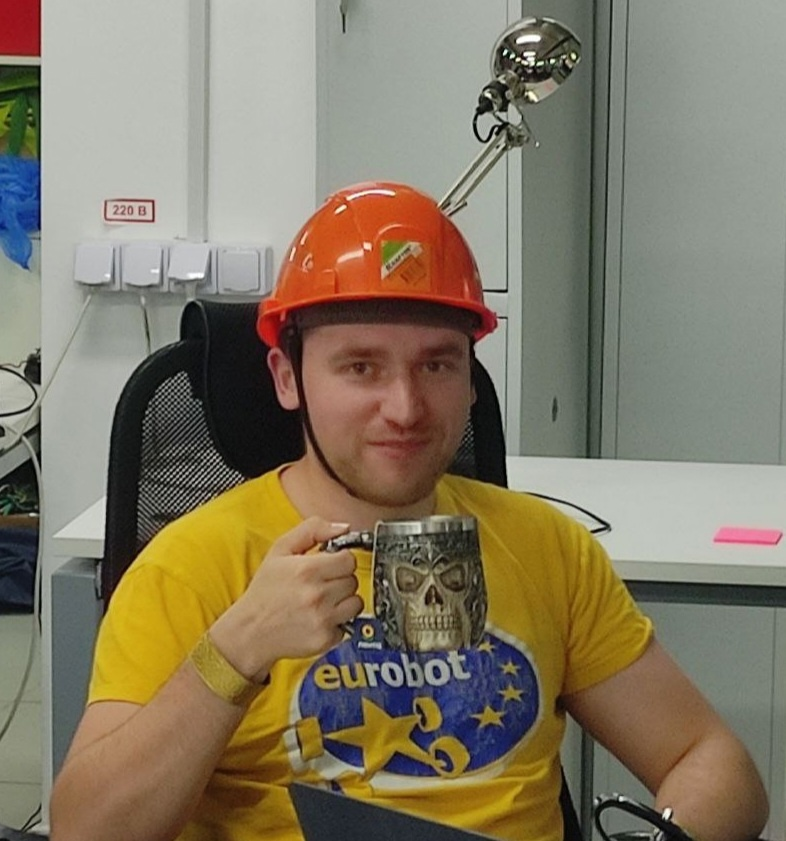
\includegraphics[height=5cm,width=1\textwidth,keepaspectratio]{Oleg.jpg}
                % \caption{caption_name}
                \label{fig:Oleg.jpg}
            \end{figure}
        \end{column}
        \begin{column}{0.49\textwidth}
            \Large
            \vspace{2cm}
            \centering
            \textbf{Oleg Bulichev} \\
            \textit{Mail}: \url{o.bulichev@innopolis.ru}\\
            \textit{TG}: \url{@Lupasic}
        \end{column}
    \end{columns}
\end{frame}

\begin{frame}[c]{Course Goal}
    \framesubtitle{}
    \centering \Large
    \textbf{To understand engineers:} \\
    their problems and \\
    their terminology \\
    \medskip
    \textit{by doing \textbf{their} job} \\
    \textit{using \textbf{their} tools}
\end{frame}

\begin{frame}[t]{Course puprose and objectives}
    \framesubtitle{}
    The development of any class of robots and the use of robots in industry requires the engineer to have knowledge and skills in:
    \begin{itemize}
        \item the ability to read engineering drawings,
        \item the analysis and synthesis of mechanisms,
        \item the dynamic calculation of mechanisms and machines,
        \item the calculation stress and strain,
        \item understanding the technological production processes,
        \item modern CAD and CAE systems.
    \end{itemize}
\end{frame}

\begin{frame}[t]{Course outline and organization}
    \framesubtitle{}
    \vspace{-0.6cm}
    \begin{figure}[H]
        \centering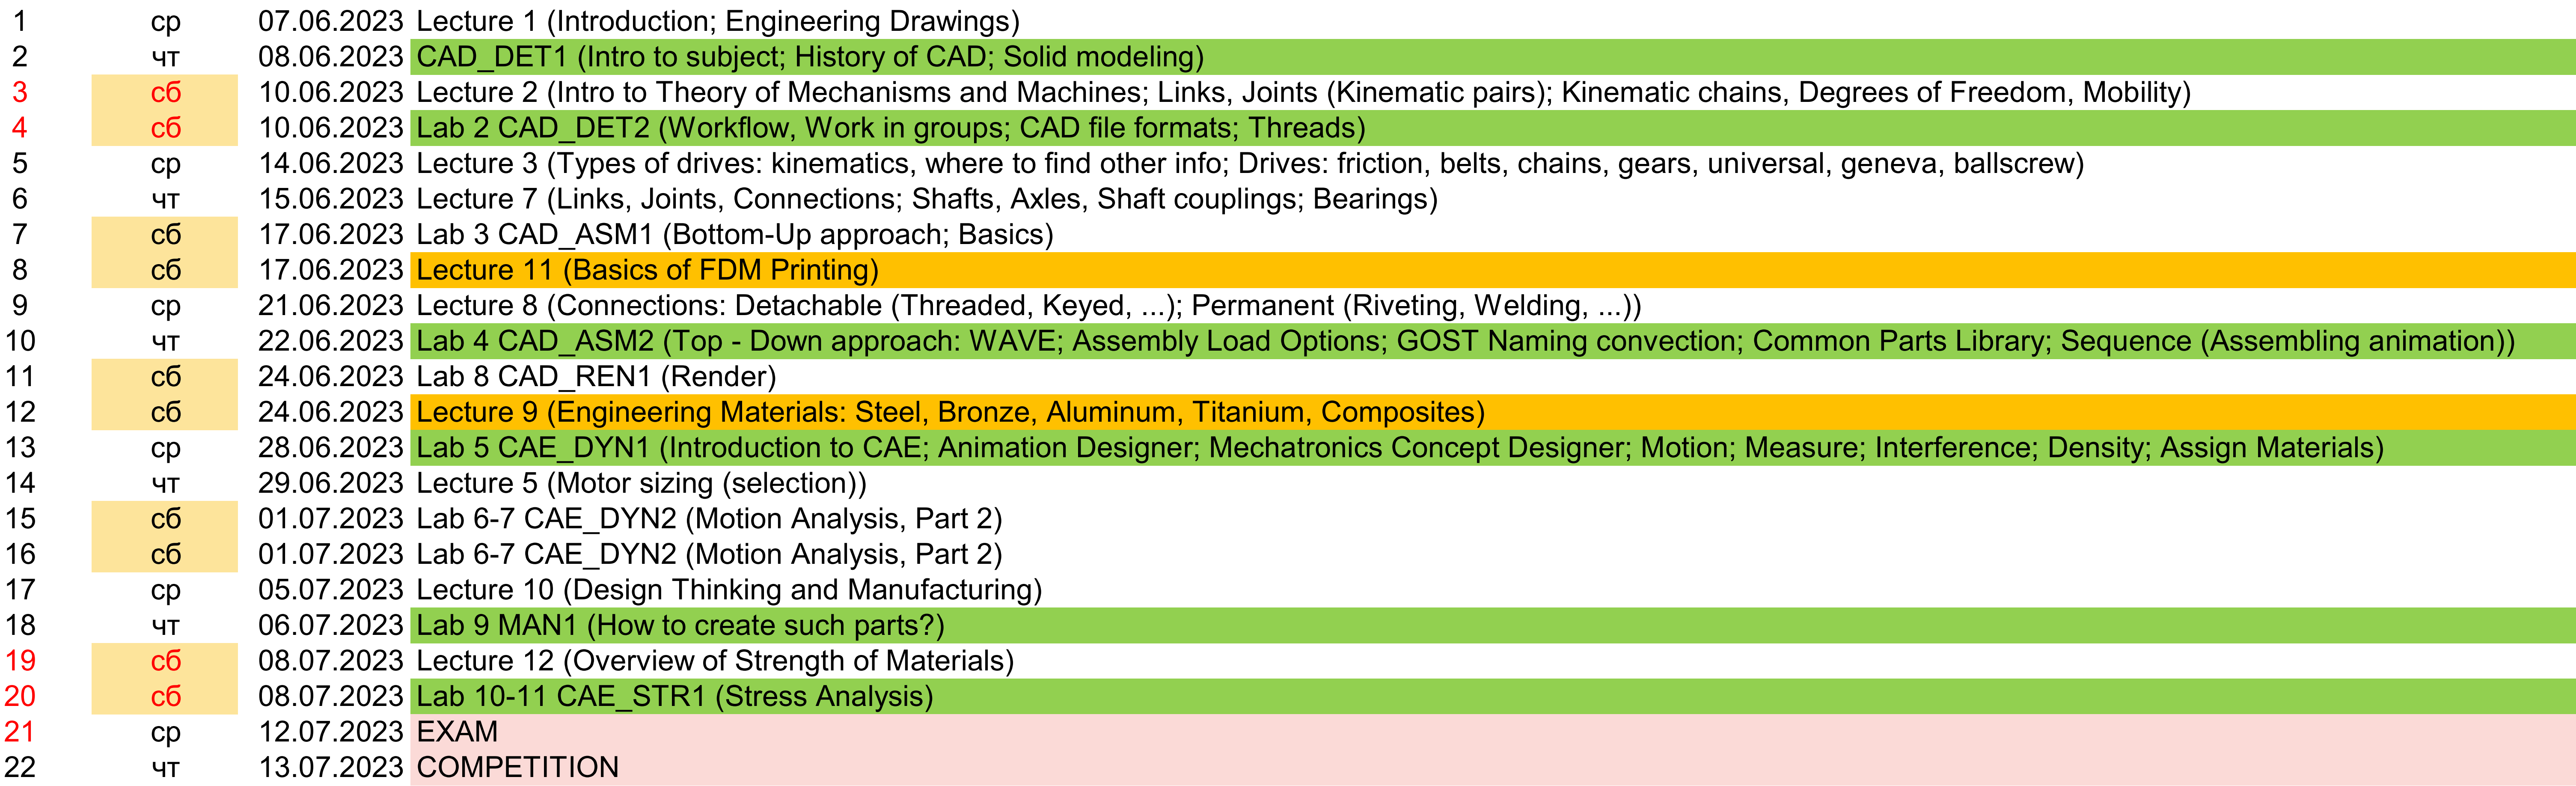
\includegraphics[height=6cm,width=1\textwidth,keepaspectratio]{topics.png}
        \label{fig:topics.png}
    \end{figure}
\end{frame}

\begin{frame}[t]{Grading criteria}
    \framesubtitle{}
    \begin{columns}[T,onlytextwidth]
        \begin{column}{0.49\textwidth}
            \textbf{What will be evaluated on the course}
            \begin{itemize}
                \item[Qz:] Quizzes: $2\times 5=10\%$ 
                \item[CP:] Competition: $20\%$
                \item[FE:] Final Exam: $30\%$
                \item[Lbs:] Lab assignments: $10\%$
                \item[HWs:] Homework assignments: $30\%$
                \item[Extra:] Slide fixes in Github: $5\%$ 
            \end{itemize}
        \end{column}
        \begin{column}{0.49\textwidth}
            \textbf{Late policy:} -100\% of max grade for a task \\
            \textbf{Scale}:
            \begin{itemize}
                \item[A:] 85 --- 100\%
                \item[B:] 70 --- 84.99\%
                \item[C:] 50 --- 69.99\%
                \item[D:] 0 --- 49.99\% or less than $50\%$ by any criterion.
            \end{itemize}
        \end{column}
    \end{columns}
\end{frame}

\begin{frame}[t]{Quizzes}
\framesubtitle{}
    \textbf{Purpose}: You will have theoretical questions on final exam. Quizzes encourage you to study material more serious.
\end{frame}

\begin{frame}[t]{Competition (Previous year)}
\framesubtitle{Bottle lifting mechanism}
    \begin{figure}[H]
        \begin{subfigure}{0.24\textwidth}
            \centering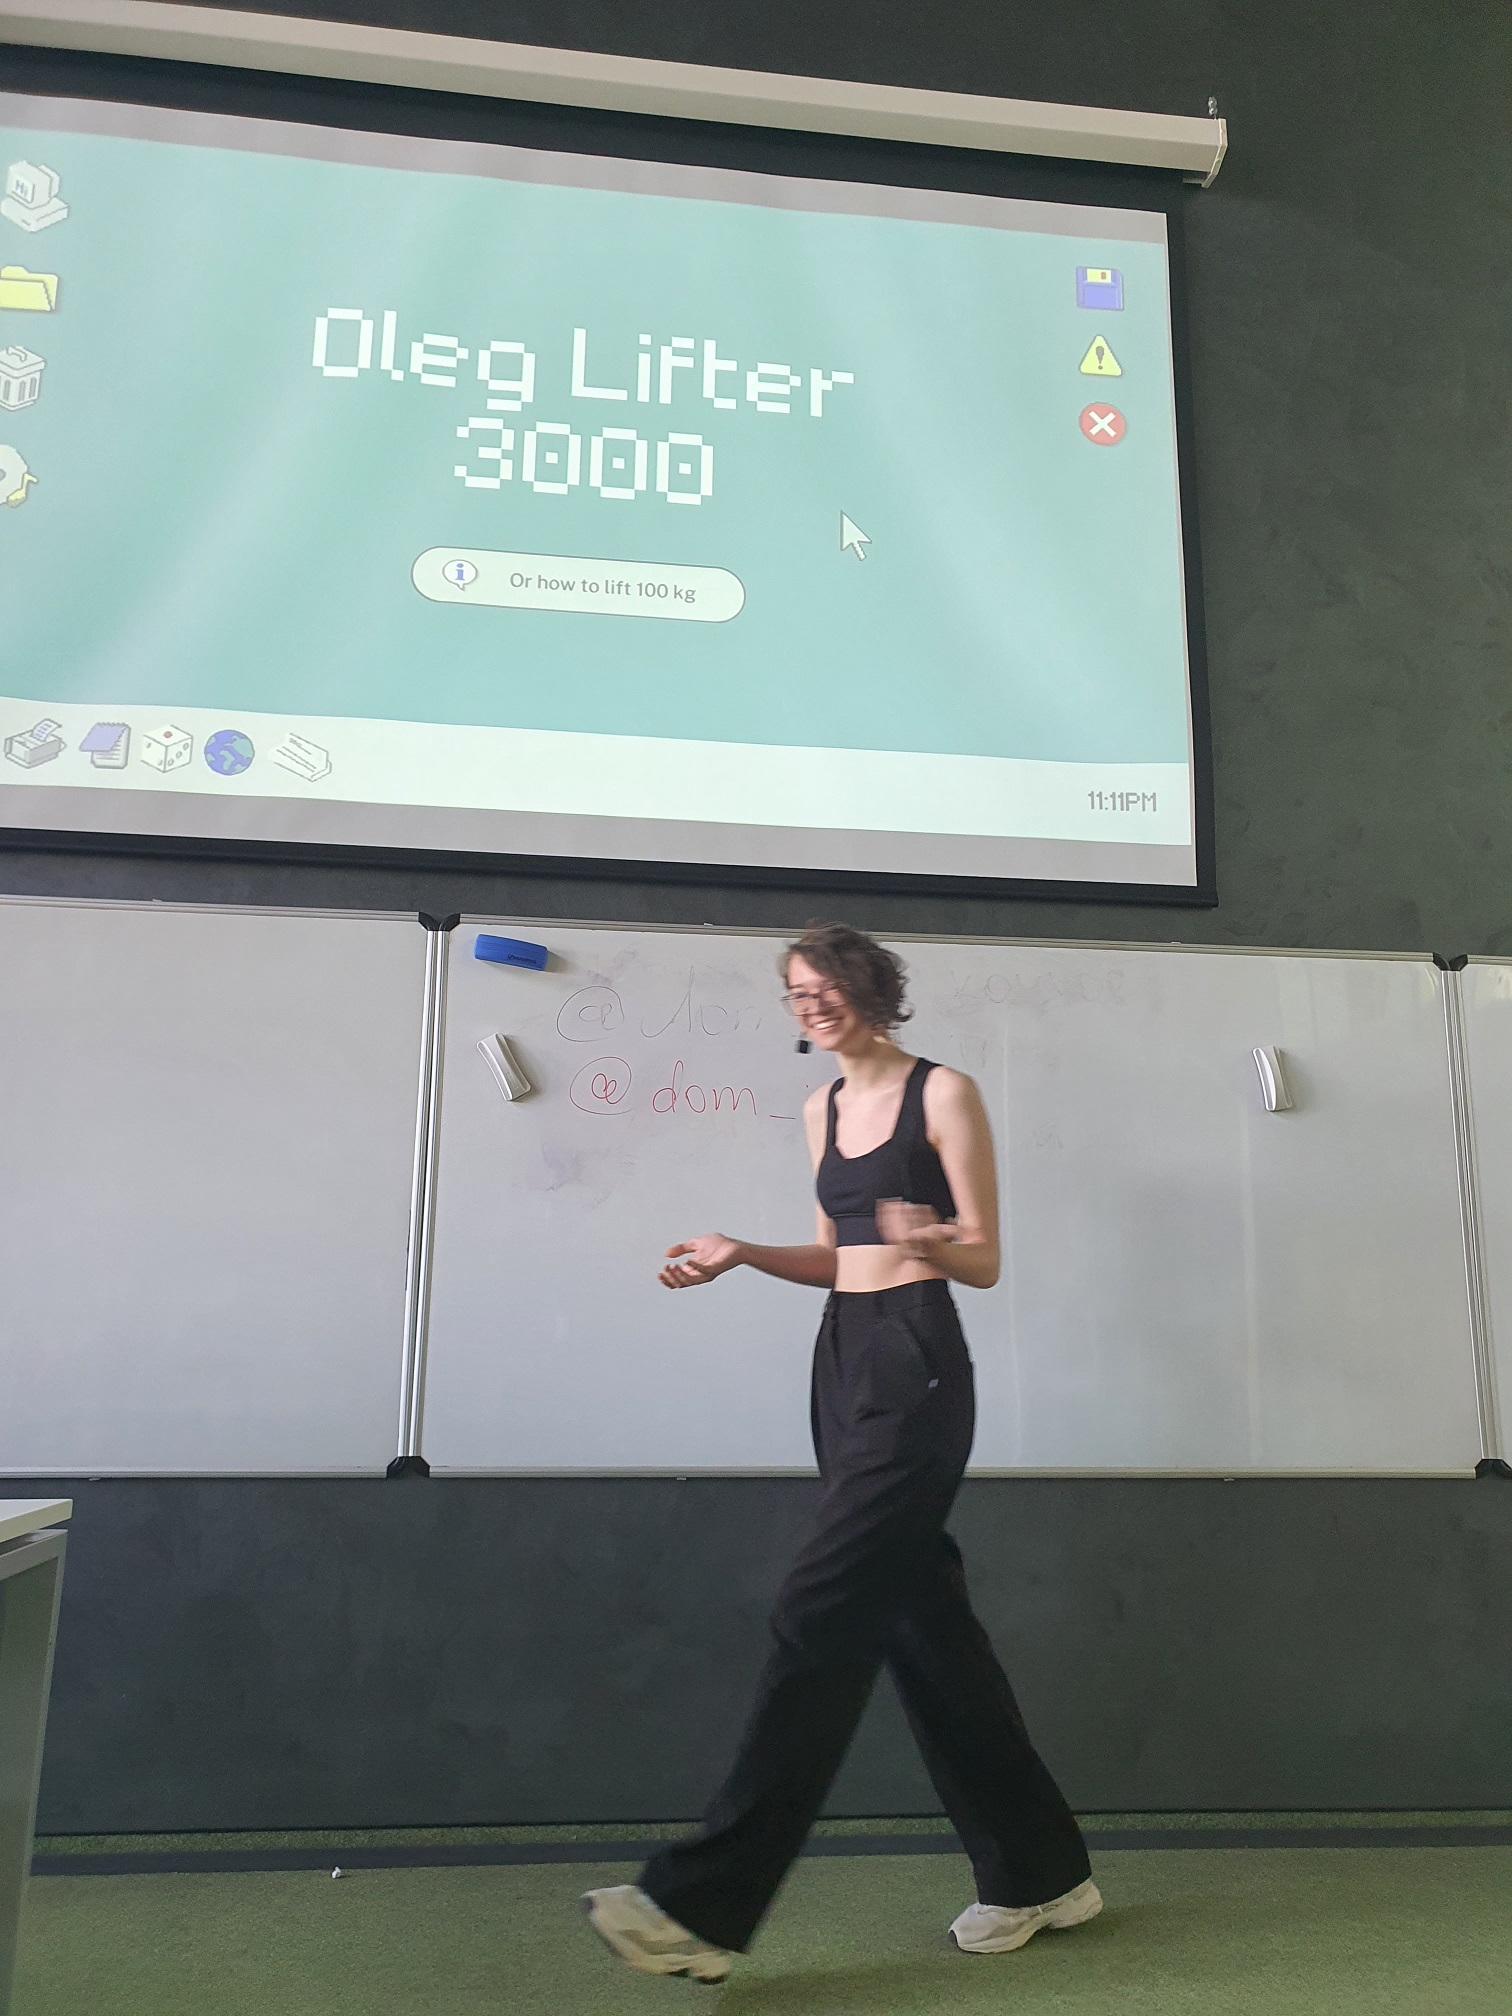
\includegraphics[height=6cm,width=1\textwidth,keepaspectratio]{2023-07-13 12-25-17.JPG}
        \end{subfigure}
        \begin{subfigure}{0.45\textwidth}
            \centering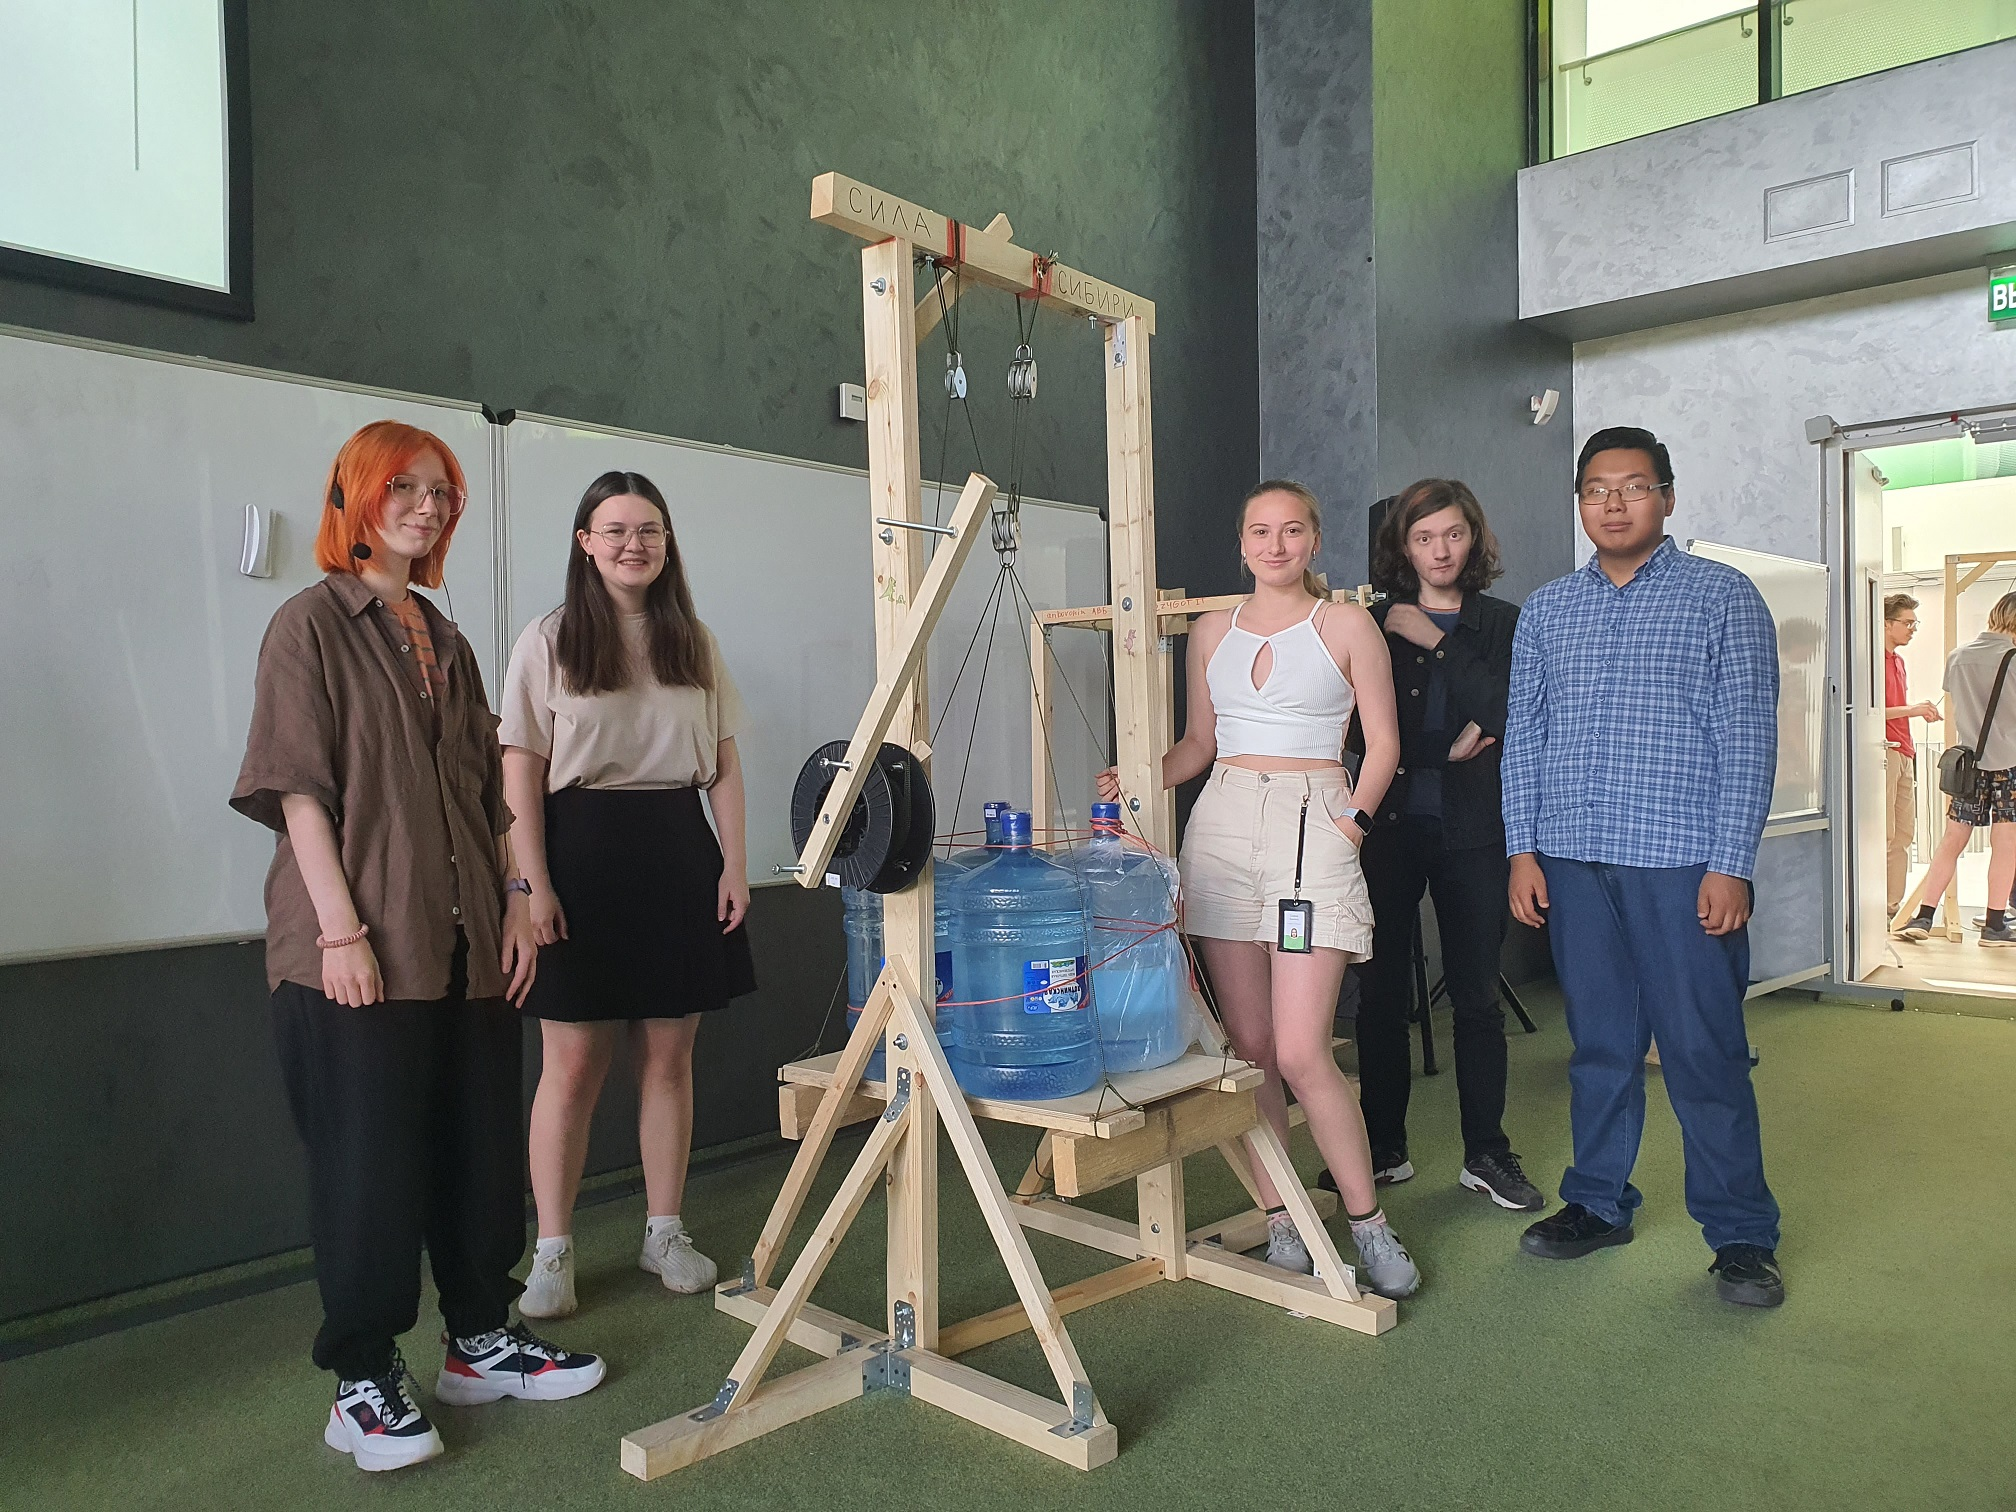
\includegraphics[height=6cm,width=1\textwidth,keepaspectratio]{2023-07-13 12-55-15.JPG}
        \end{subfigure}
        \begin{subfigure}{0.24\textwidth}
            \centering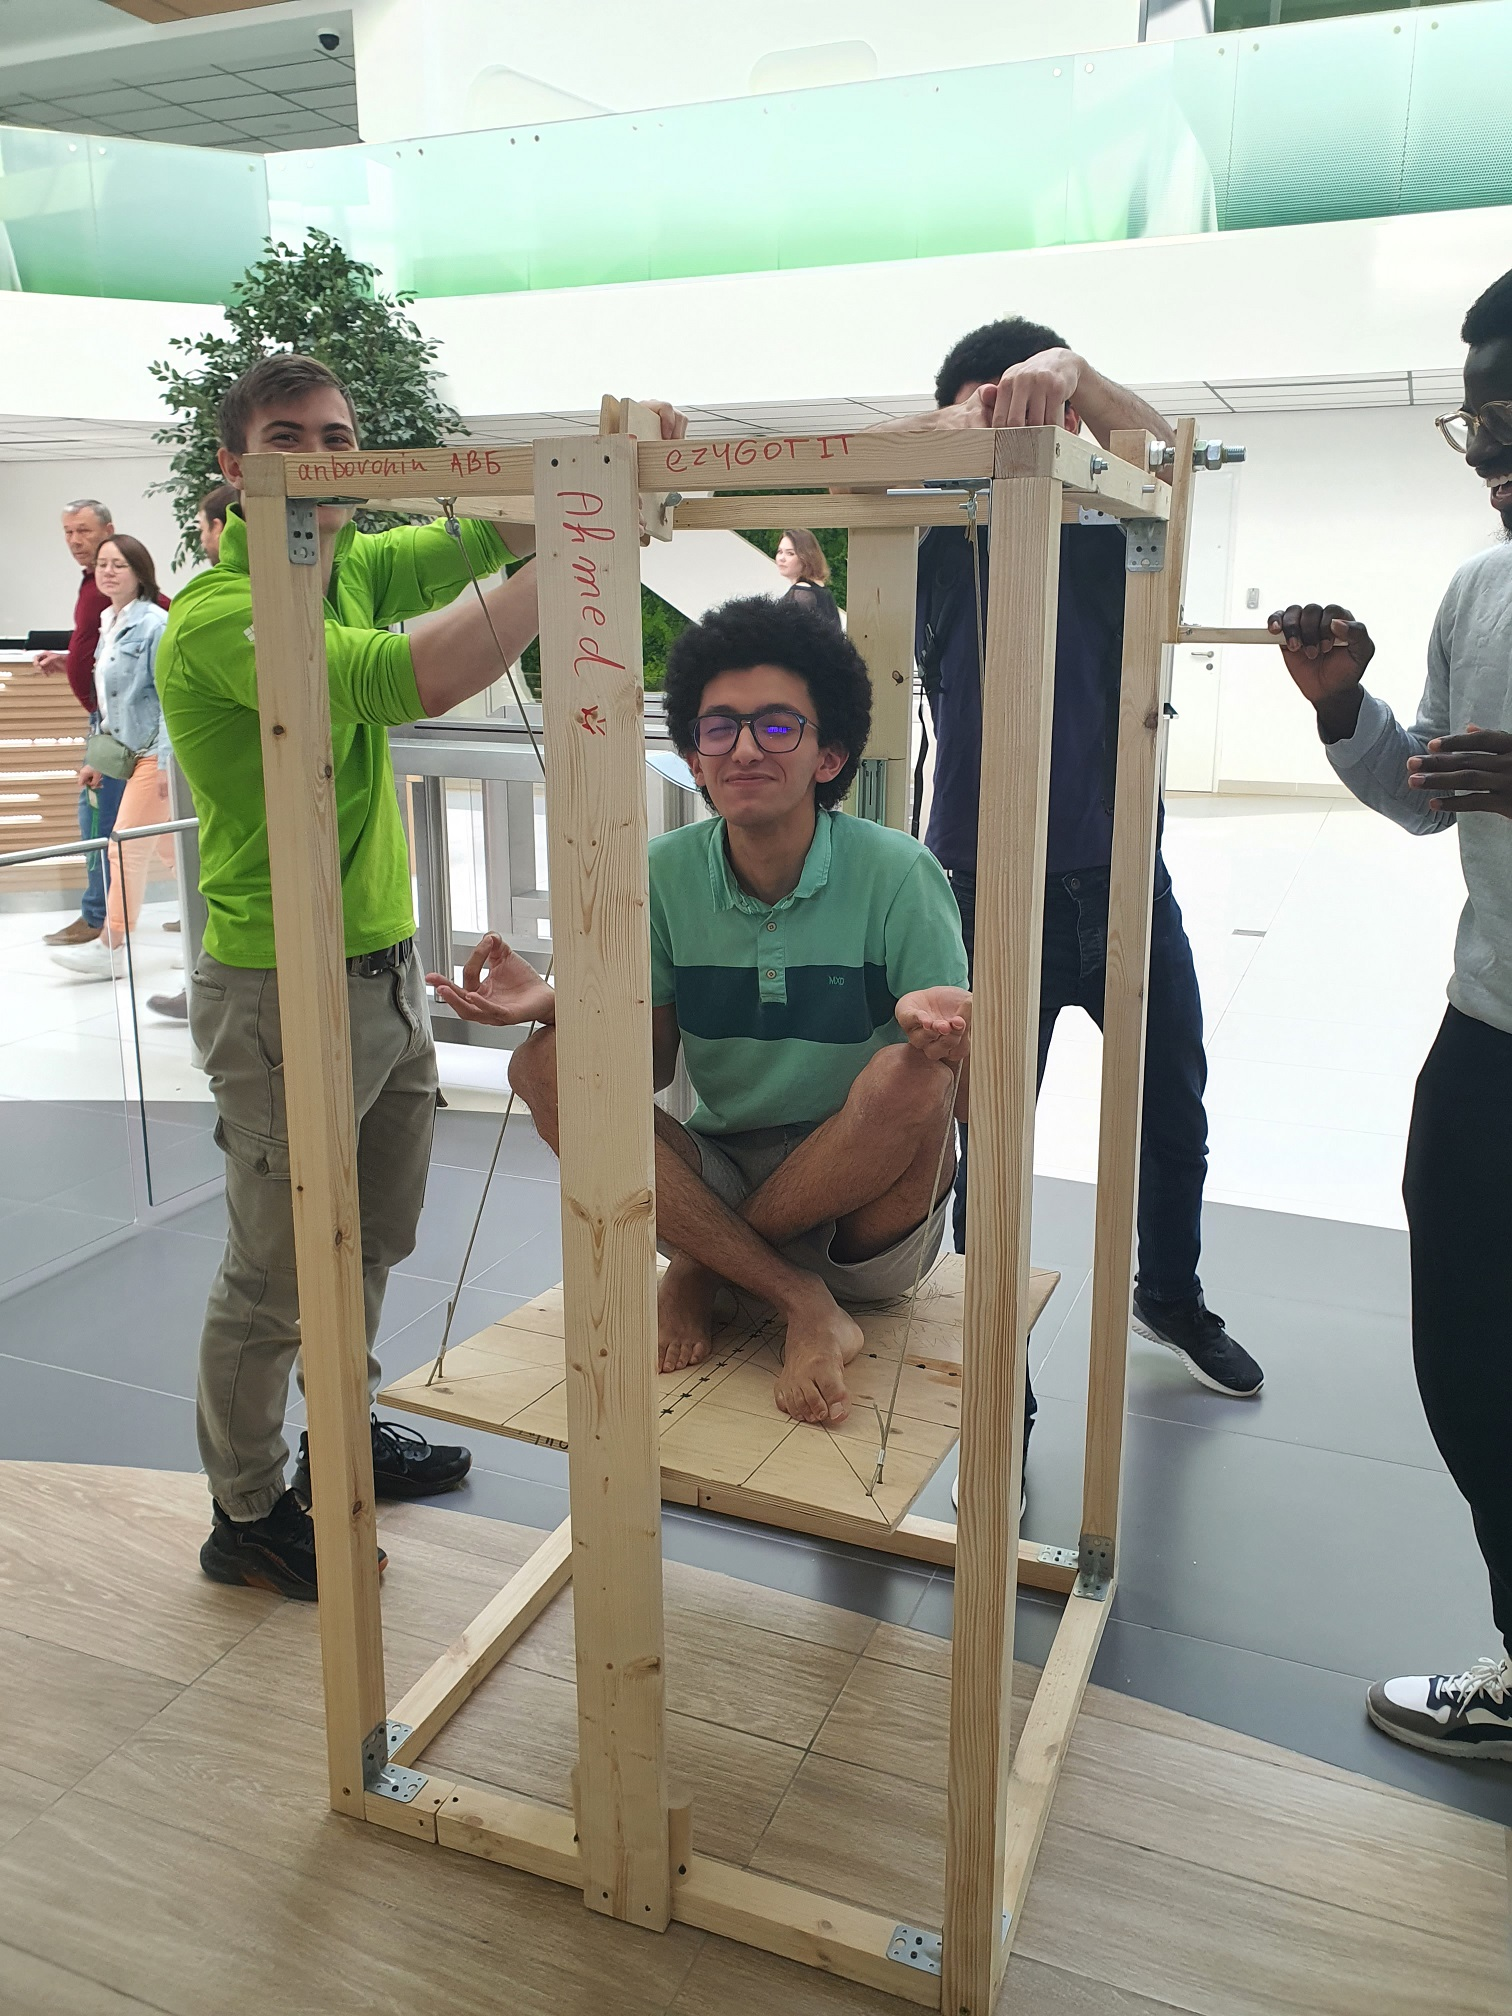
\includegraphics[height=6cm,width=1\textwidth,keepaspectratio]{2023-07-13 13-25-20.JPG}
        \end{subfigure}
    \end{figure}
\end{frame}

\begin{frame}[c]{Competition: Let's vote}
    \framesubtitle{}
    \vspace{-0.6cm}
    \begin{figure}[H]
        \begin{subfigure}[t]{0.32\textwidth}
            \centering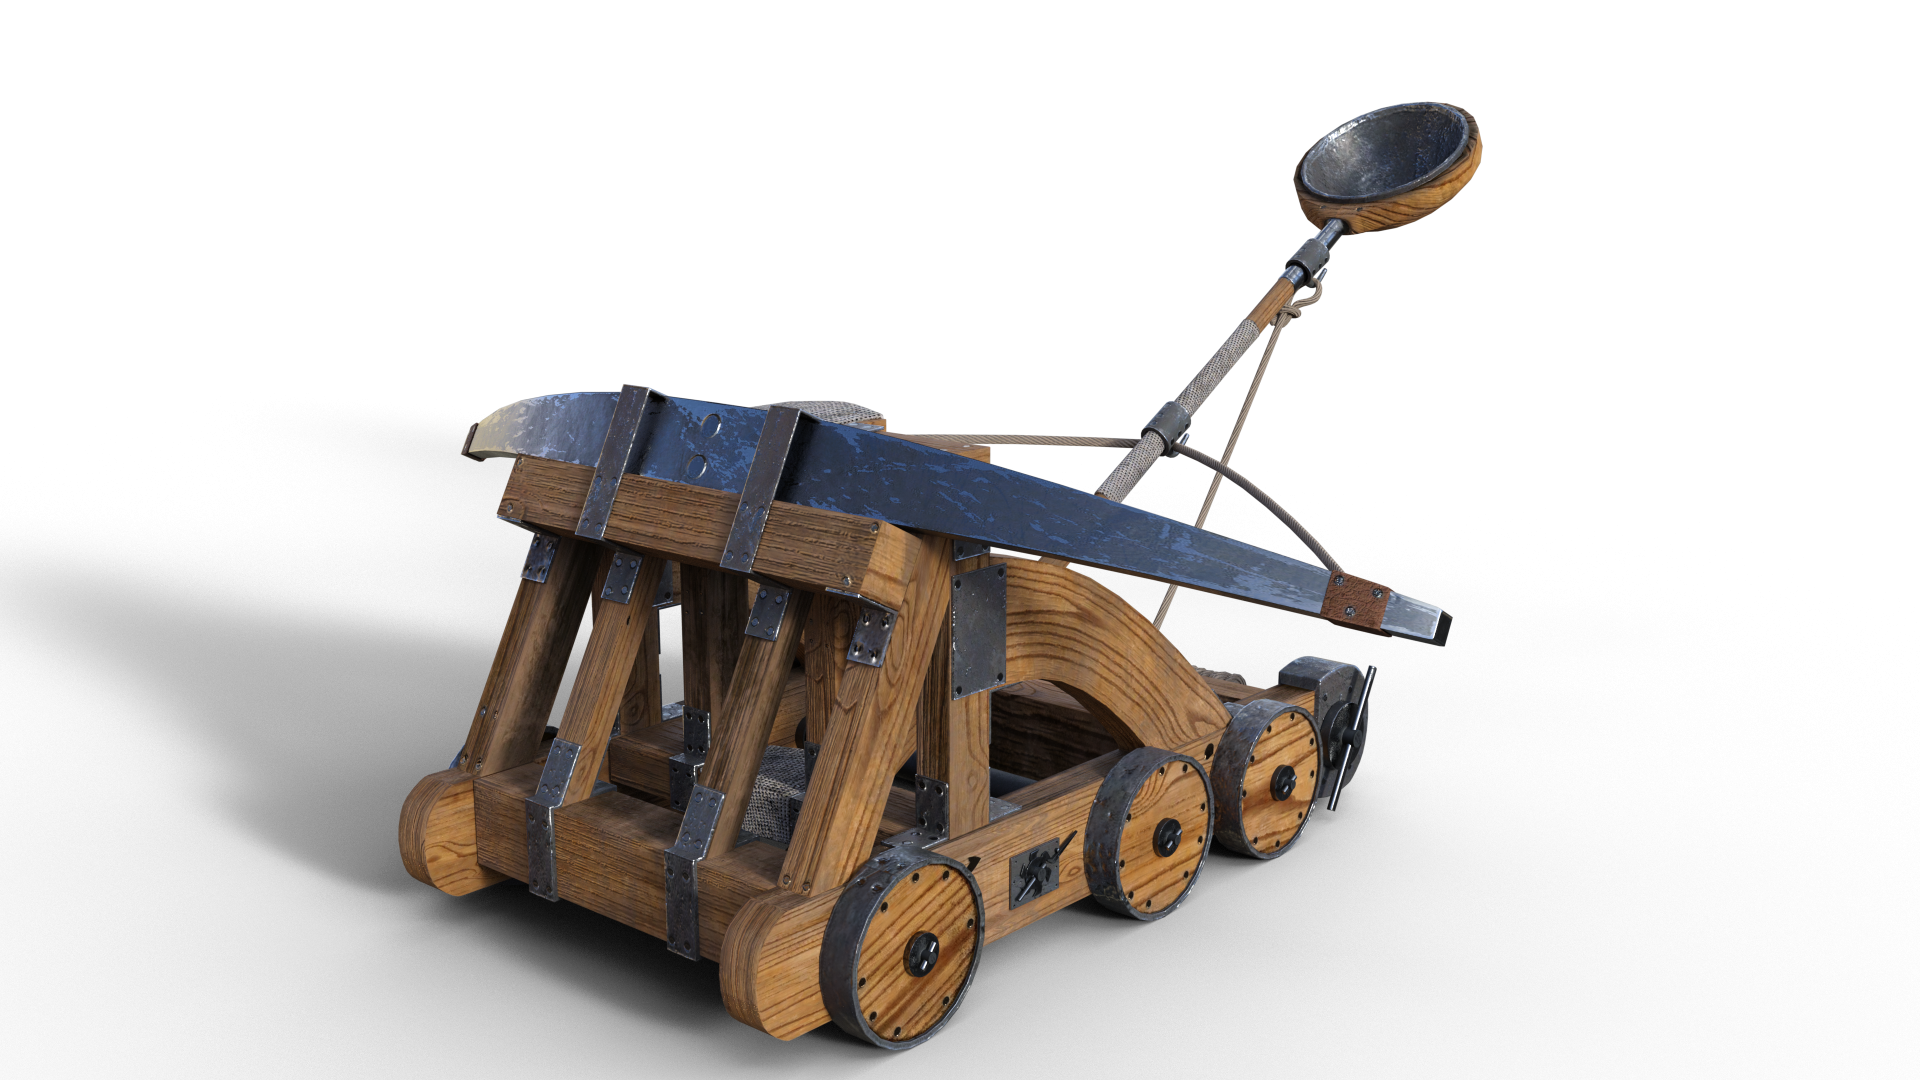
\includegraphics[height=2.5cm,width=1\textwidth,keepaspectratio]{catapuylt.png}
            \caption{\textbf{Ball throwing mechanism}}
            \label{fig:catapuylt.png}
        \end{subfigure}
        \begin{subfigure}[t]{0.32\textwidth}
            \centering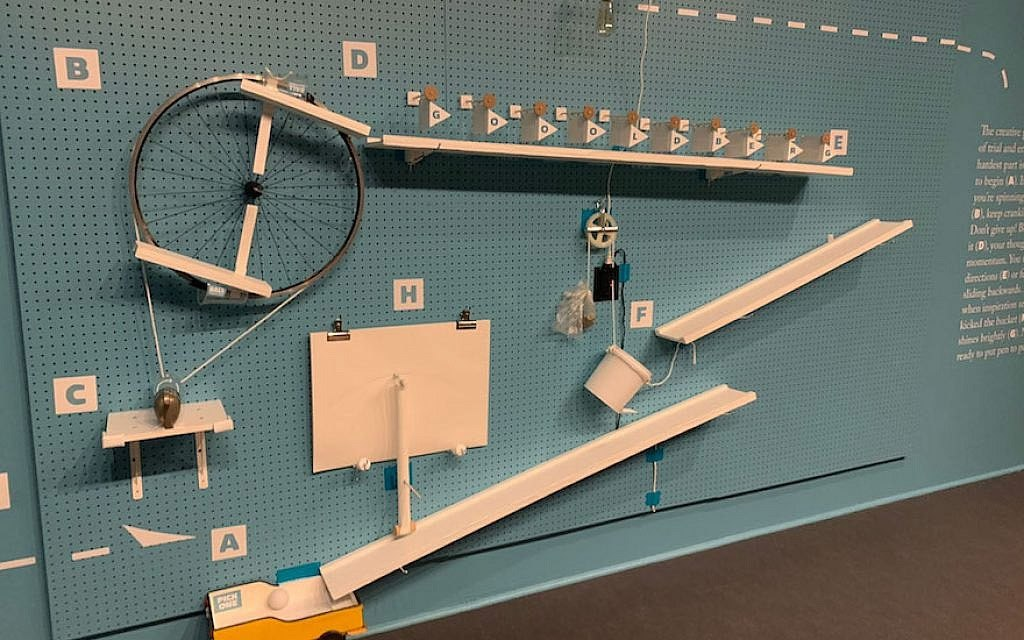
\includegraphics[height=2.5cm,width=1\textwidth,keepaspectratio]{overengineering.jpg}
            \caption{\textbf{Bizarre Teabag dropper}}
            \label{fig:overengineering.jpg}
        \end{subfigure}
        \begin{subfigure}[t]{0.32\textwidth}
            \centering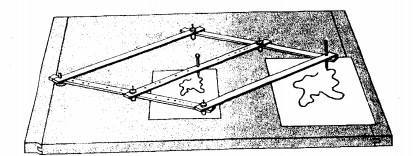
\includegraphics[height=2.5cm,width=1\textwidth,keepaspectratio]{copycat.jpeg}
            \caption{\textbf{Image copier}}
            \label{fig:copycat.jpeg}
        \end{subfigure}

        \begin{subfigure}[t]{0.49\textwidth}
            \centering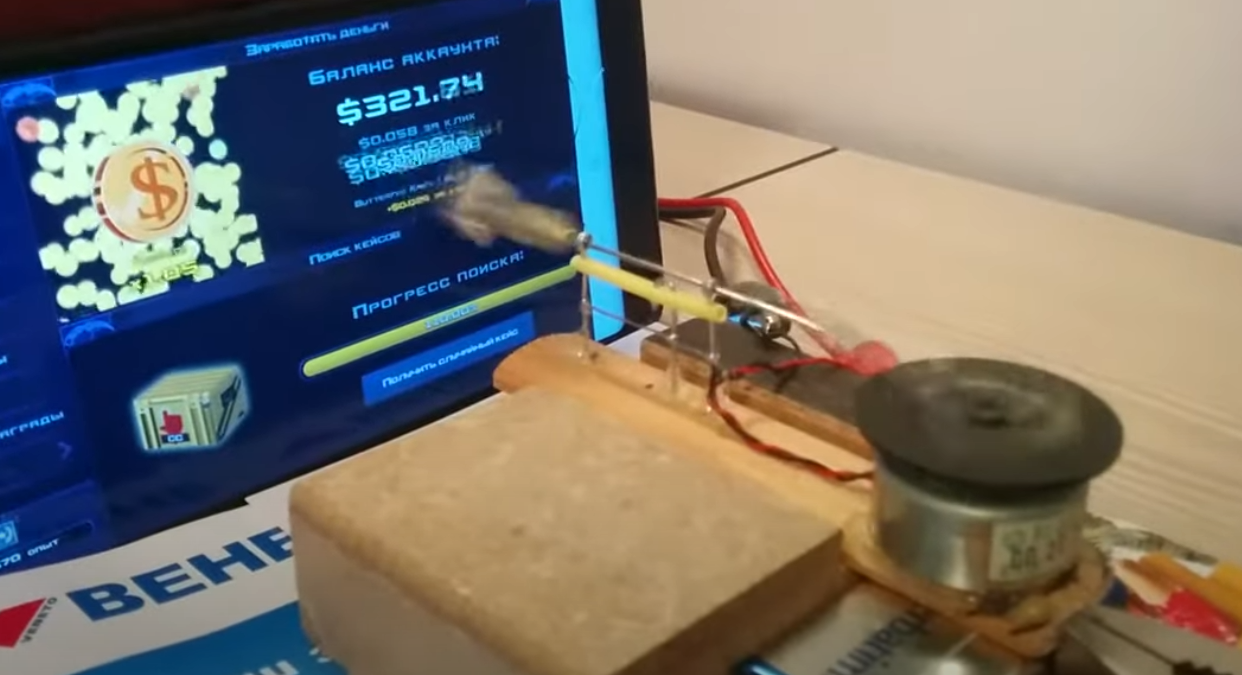
\includegraphics[height=2.5cm,width=1\textwidth,keepaspectratio]{2024-06-04_23-36-11.png}
            \caption{\textbf{Autoclicker for smartphone games}}
        \end{subfigure}
        \begin{subfigure}[t]{0.49\textwidth}
            \centering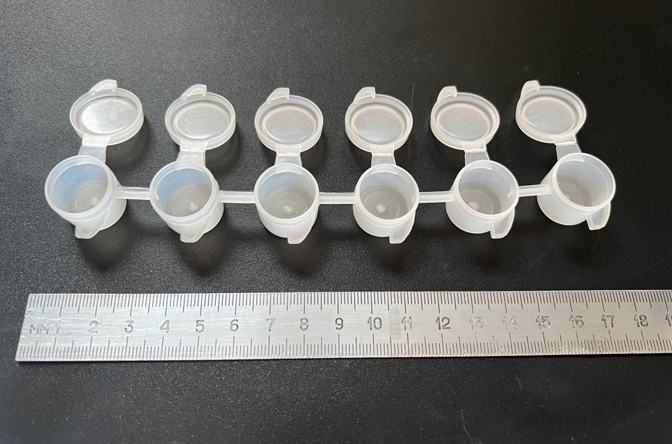
\includegraphics[height=2.5cm,width=1\textwidth,keepaspectratio]{2024-06-04_23-34-01.png}
            \caption{\textbf{Closing mechanism for paint cans}}
        \end{subfigure}
    \end{figure}
\end{frame}

\begin{frame}[t]{Final Exam (Previous Year)}
    \framesubtitle{}
        \begin{figure}[H]
            \begin{subfigure}{0.32\textwidth}
                \centering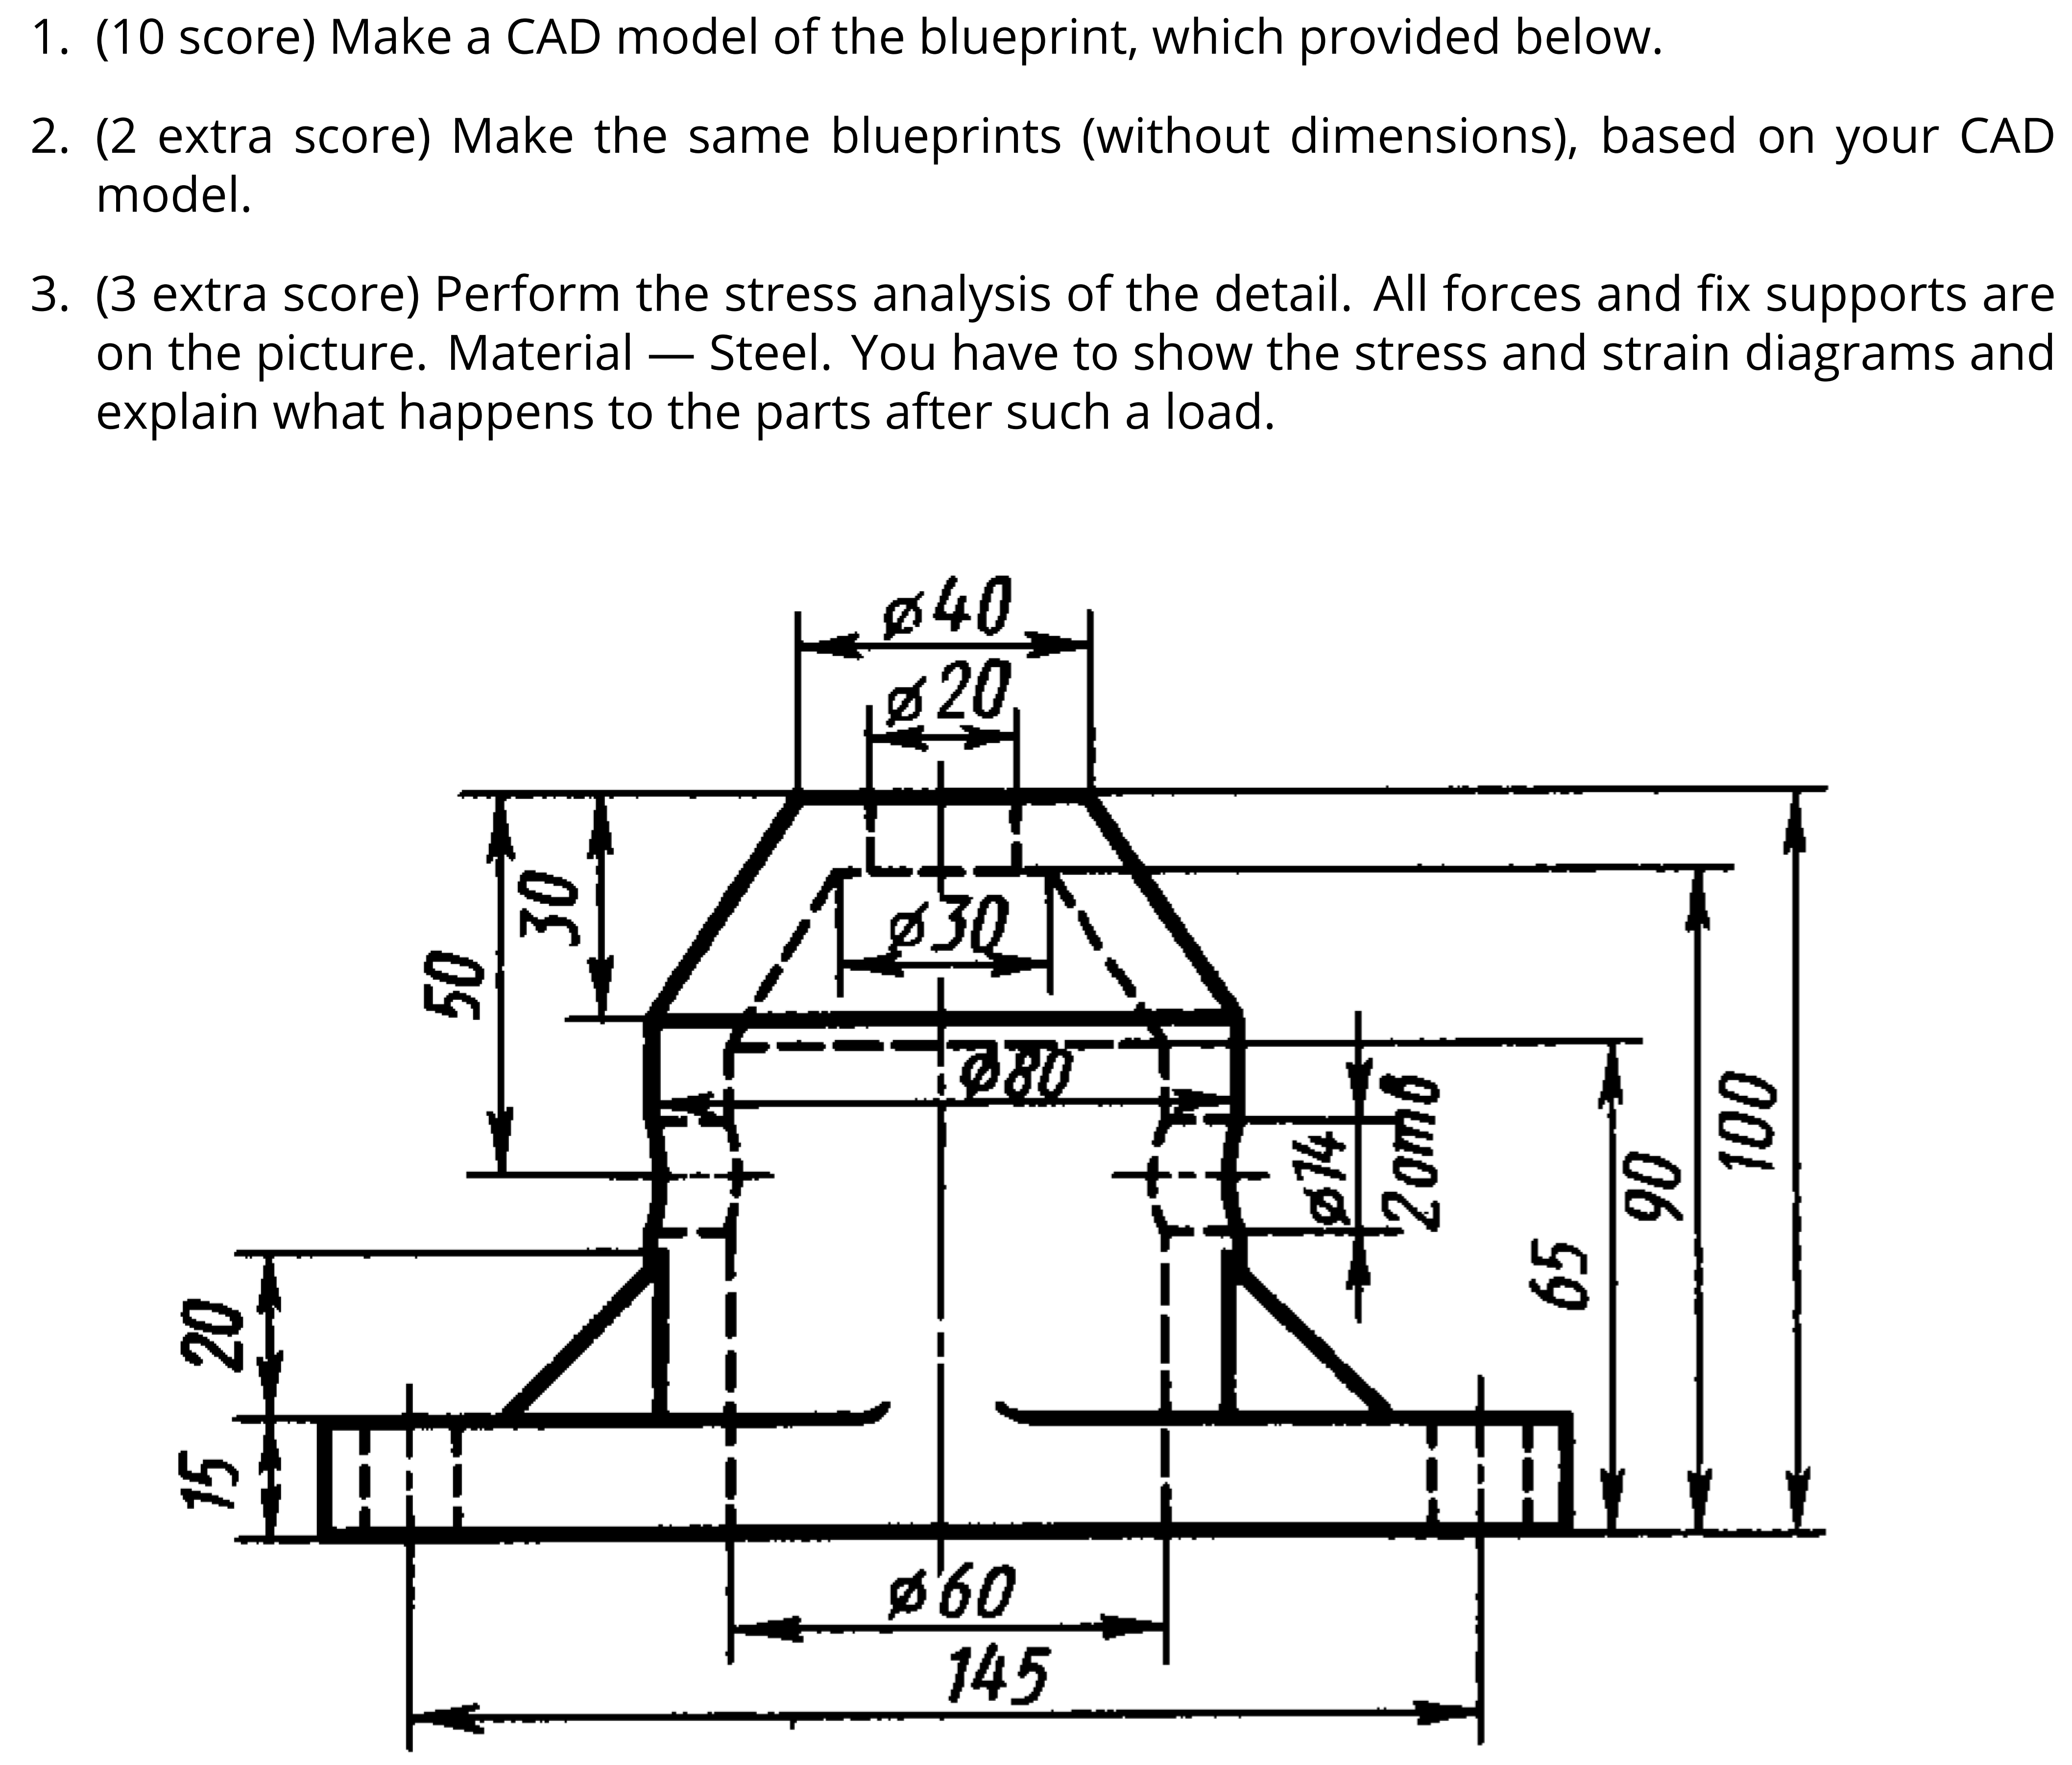
\includegraphics[height=6cm,width=1\textwidth,keepaspectratio]{resources/ex1.png}
                \caption*{CAD part}
                \label{fig:resources/ex1.png}
            \end{subfigure}
            \begin{subfigure}{0.32\textwidth}
                \centering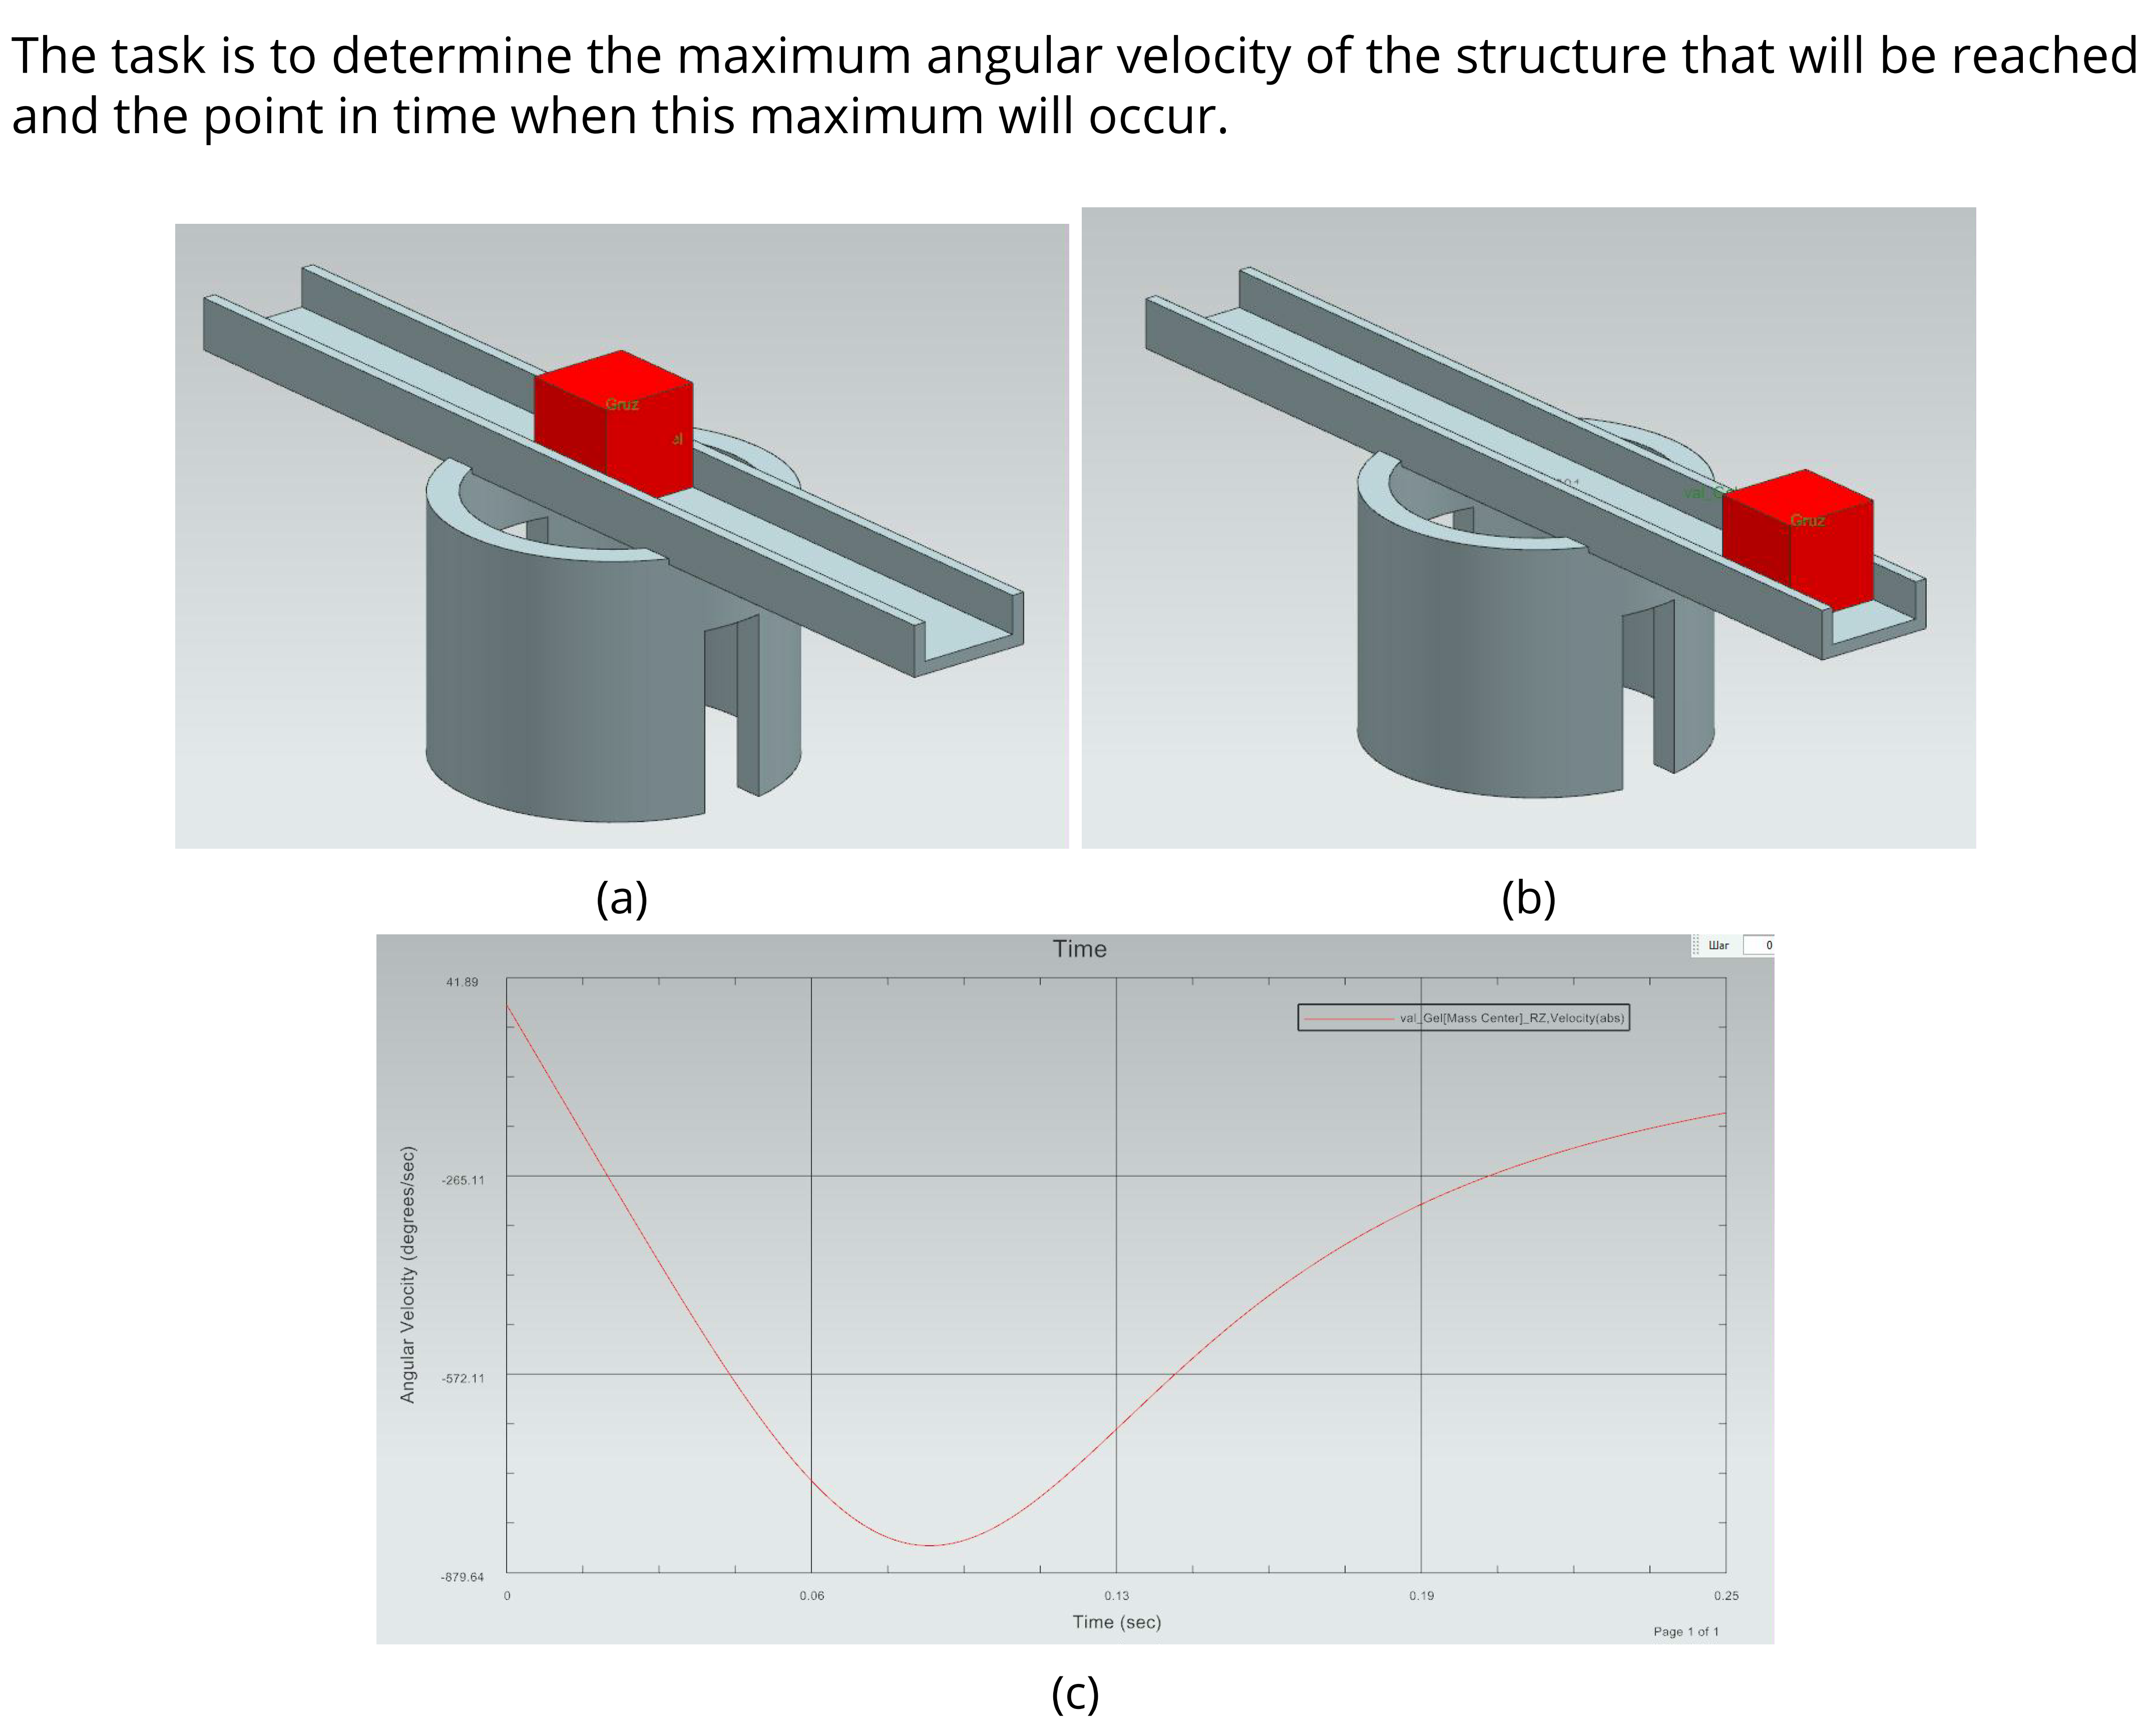
\includegraphics[height=6cm,width=1\textwidth,keepaspectratio]{resources/ex2.png}
                \caption*{CAE part}
                \label{fig:resources/ex2.png}
            \end{subfigure}
            \begin{subfigure}{0.32\textwidth}
                \centering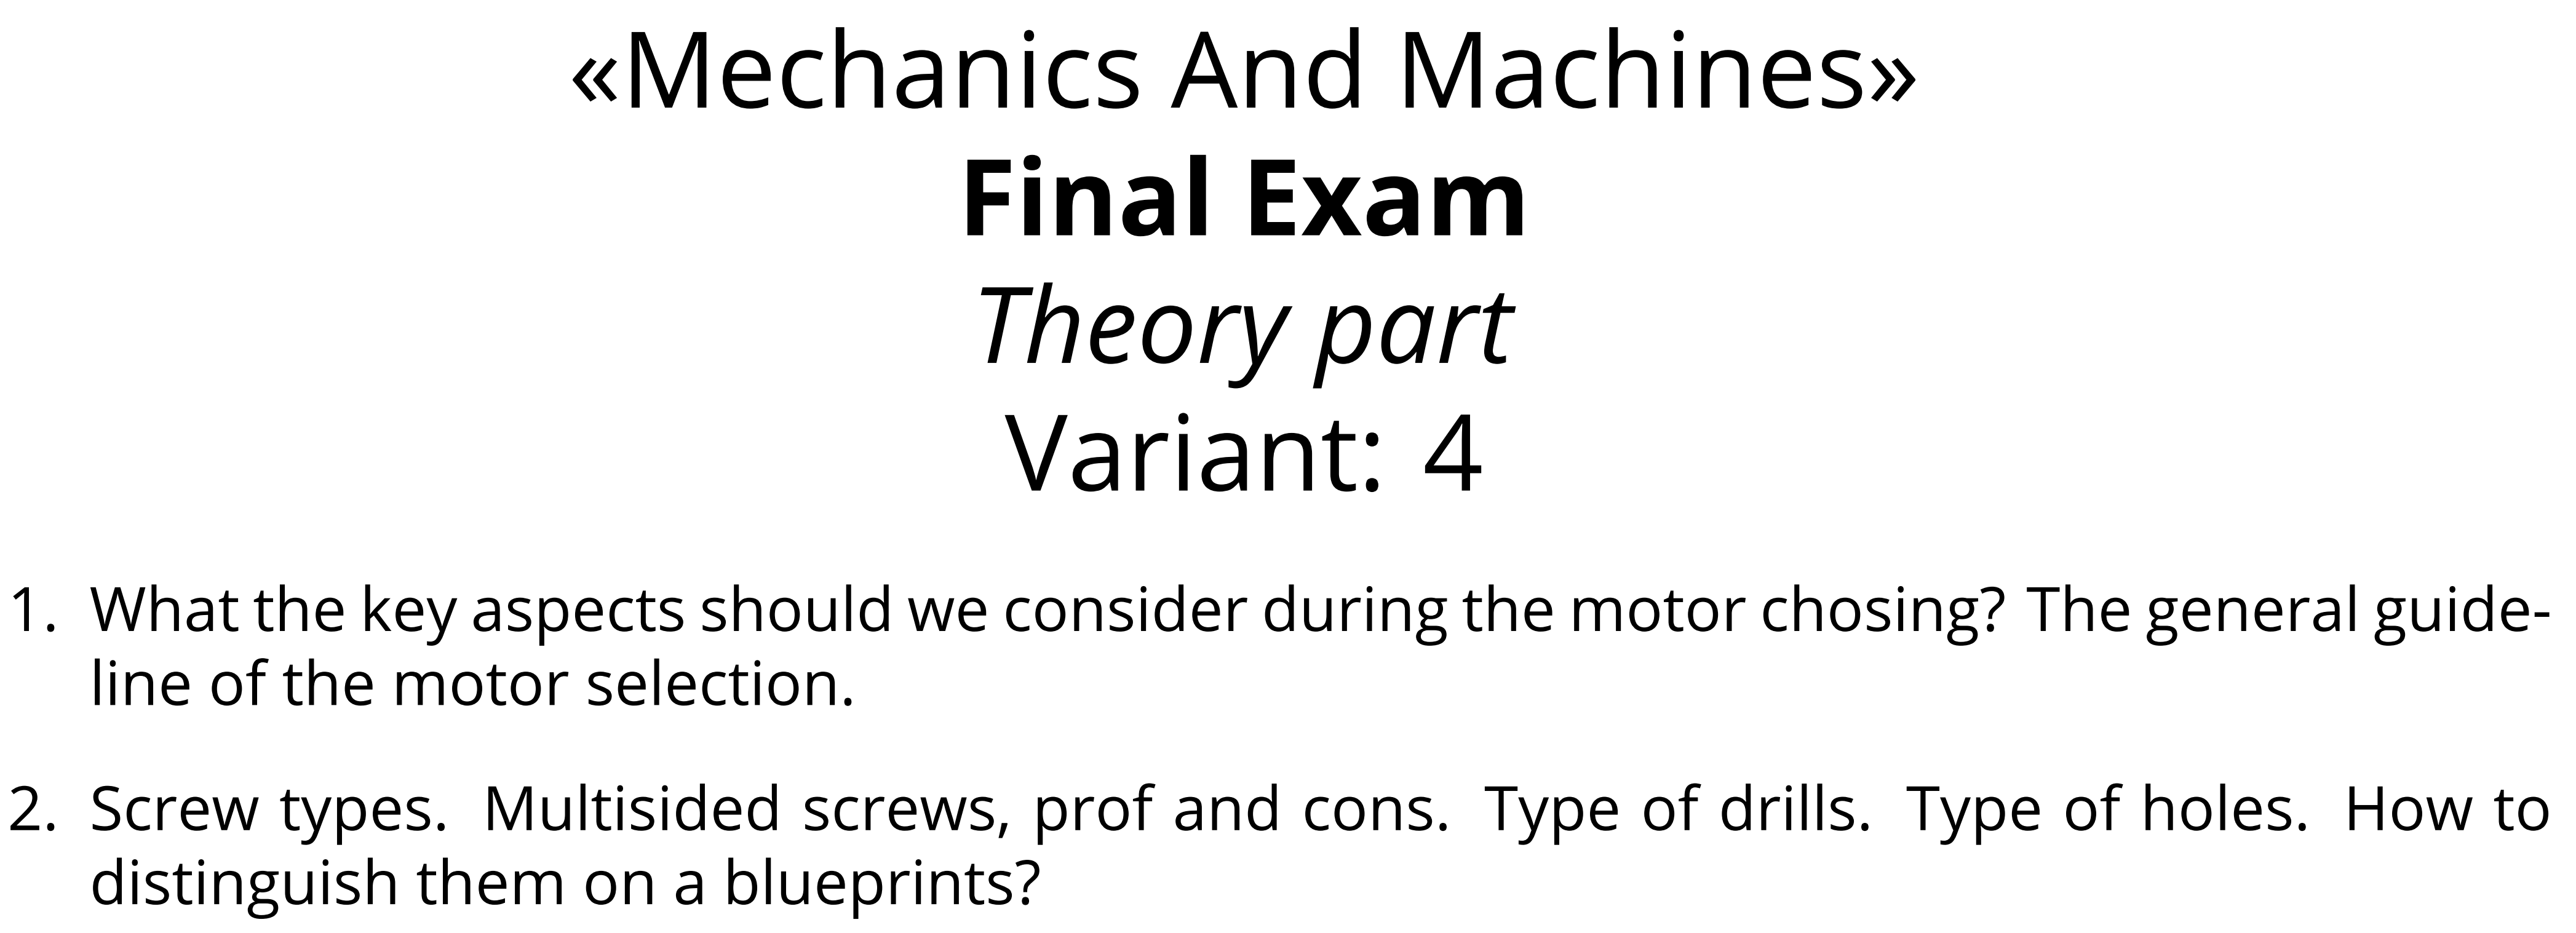
\includegraphics[height=6cm,width=1\textwidth,keepaspectratio]{resources/ex3.png}
                \caption*{Theory part}
                \label{fig:resources/ex3.png}
            \end{subfigure}
        \end{figure}
    \end{frame}

\begin{frame}[c]{}
    \framesubtitle{}
    \centering \LARGE \textbf{Lab Goals} \\
    To obtain the needed tools for solving the design part of the competition
\end{frame}

\begin{frame}[t]{Computer Aided Design}
    \framesubtitle{}
        \vspace{-0.6cm}
        \begin{figure}[H]
            \centering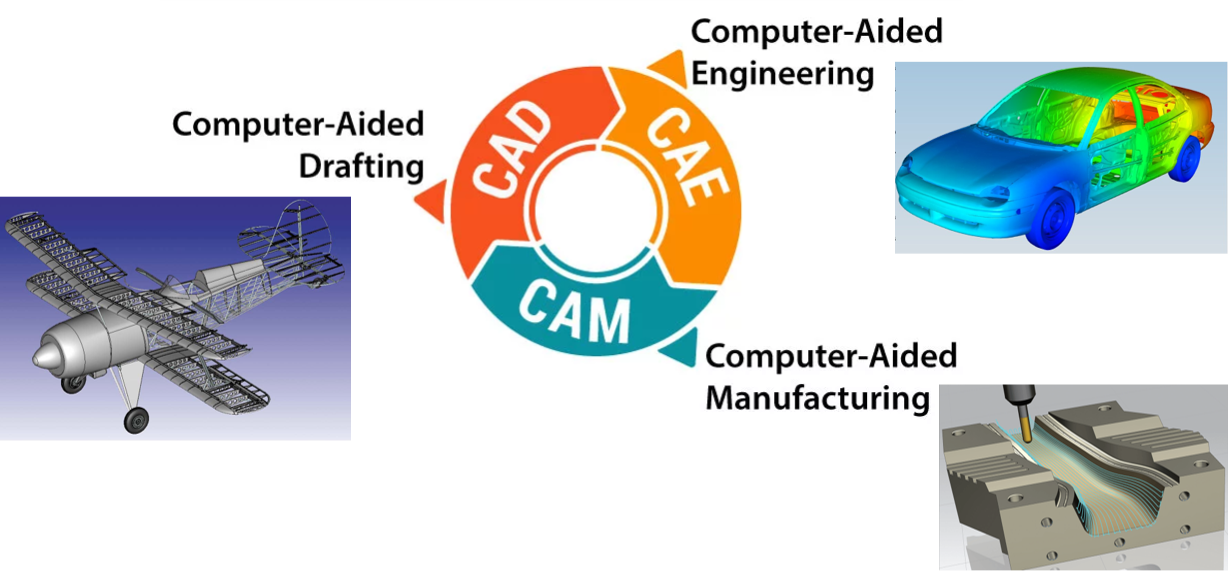
\includegraphics[height=6.5cm,width=1\textwidth,keepaspectratio]{resources/CADCAMCAE.png}
            \label{fig:resources/CADCAMCAE.png}
        \end{figure}
    \end{frame}
    
    \begin{frame}[t]{Computer Aided Design}
    \framesubtitle{Types of modeling}
        \vspace{-0.6cm}
        \begin{figure}[H]
            \centering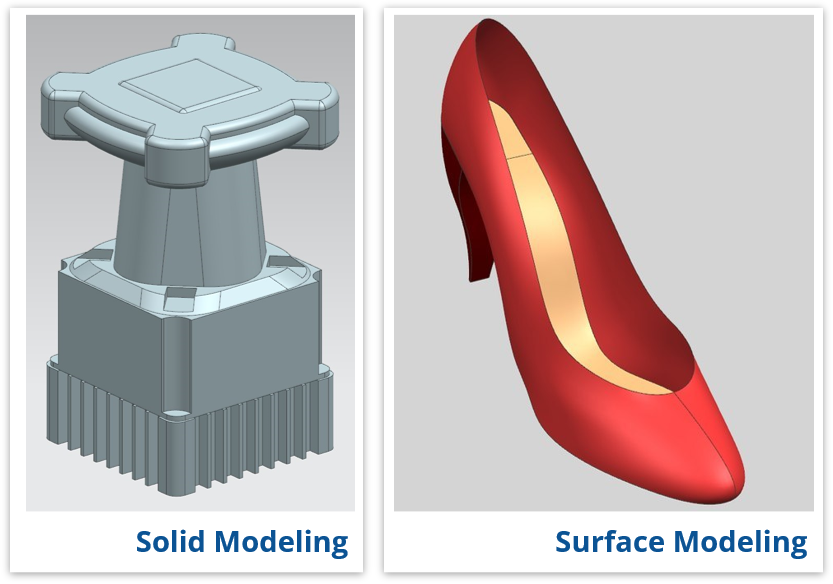
\includegraphics[height=6cm,width=1\textwidth,keepaspectratio]{resources/solidsurface.png}
            \label{fig:resources/solidsurface.png}
        \end{figure}
    \end{frame}
    
    \begin{frame}[t]{History of CAD}
    \framesubtitle{}
        \begin{itemize}
            \item[60th] --- Theoretical studies of the possibility of solving design problems on the computer were carried out.
            \item[70th] --- Methods, algorithms and programs for solving individual tasks for different design stages were developed.
            \item[80th] --- CAD is being developed and improved. 3D modeling became more popular.
            \item[90th] --- Developers had finished formation of base concepts of CAD and unified data transfer between systems.
        \end{itemize}
    \end{frame}
    
    \begin{frame}[c]{}
        \framesubtitle{}
            \LARGE\centering
            \textbf{CAD benefits}\\
            \medskip
            Cheaper\\
            Safer \\
            Faster
        \end{frame}
    
    \begin{frame}[c]{Popular CAD systems in Russia}
    \framesubtitle{}
        \vspace{-0.6cm}
        \begin{figure}[H]
            \centering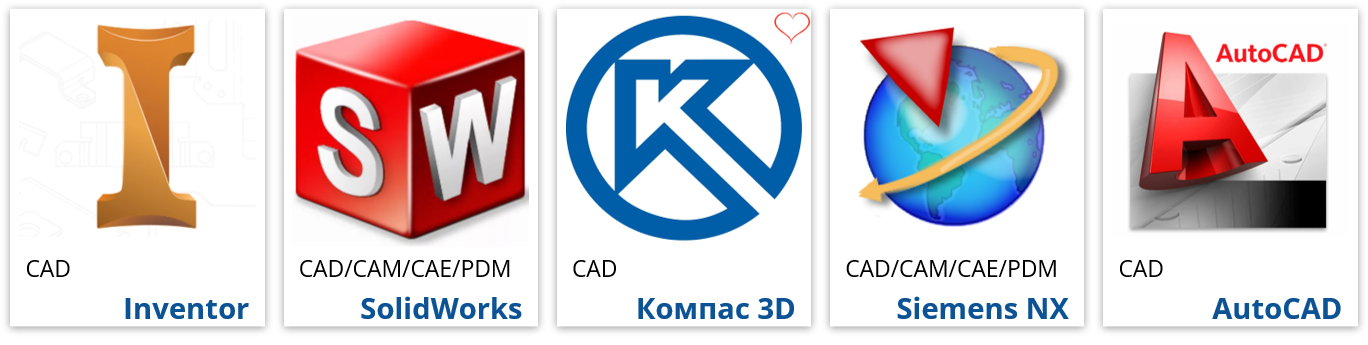
\includegraphics[height=6.5cm,width=1\textwidth,keepaspectratio]{resources/CADs.png}
            \label{fig:resources/CADs.png}
        \end{figure}
    \end{frame}
    
    \begin{frame}[t]{Siemens NX}
    \framesubtitle{}
        \begin{columns}[T,onlytextwidth]
            \begin{column}{0.32\textwidth}
                \centering\textbf{Prof}
                \begin{itemize}
                    \item All in one system (CAD,CAM,CAE,PDM)
                    \item Free for students
                    \item Can create a real aircraft in it
                \end{itemize}
            \end{column}
            \begin{column}{0.32\textwidth}
                \begin{figure}[H]
                    \centering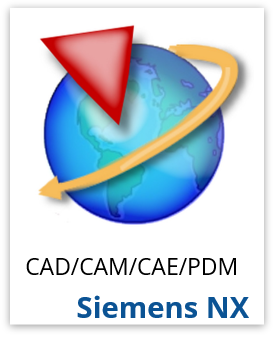
\includegraphics[height=6cm,width=1\textwidth,keepaspectratio]{resources/NXpic.png}
                    % \caption{caption_name}
                    \label{fig:resources/NXpic.png}
                \end{figure}
            \end{column}
            \begin{column}{0.32\textwidth}
                \centering\textbf{Cons}
                \begin{itemize}
                    \item Complex system
                    \item Not popular in small companies
                \end{itemize}
            \end{column}
        \end{columns}
    \end{frame}
    
    \begin{frame}[t]{Common usage of other systems for our tasks}
    \framesubtitle{}
        \begin{itemize}
            \item If you need a good drawings. Make CAD anywhere, afterwards import to Kompas-3D.
            \item If you need Standard Component Library (SCL), use either Kompas, or Solid Edge, or \href{https://www.mcmaster.com/}{mcmaster}. Insert needed stuff in NX.
        \end{itemize}
    \end{frame}

\begin{frame}[t]{Common Labs Workflow}
\framesubtitle{}
\vspace{-0.4cm}

    \textbf{Lab 1}
    \begin{enumerate}
        \scriptsize
        \item Oleg explains some new concepts.
        \item Oleg provides HW, which should be done after the lab.
        \item You start to watch prerecorded videos and make class tasks. You can do it at home.
    \end{enumerate}
    \textbf{Between lab 1 and lab 2}
    \begin{enumerate}
        \scriptsize
        \item You should finish lab tasks and solve HW.
        \item Submit only HW in Moodle.
    \end{enumerate}
    \textbf{Lab 2}
    \begin{enumerate}
        \scriptsize
        \item Oleg explains some new concepts.
        \item Oleg provides new HW, which should be done after the lab.
        \item If you had self-study lectures --- Oleg conducts quiz.
        \item You defend previous lab task solutions and HW results.
        \item You start to watch prerecorded videos and make class tasks. You can do it at home.
    \end{enumerate}
\end{frame}

\begin{frame}[c]{}
    \framesubtitle{}
    \LARGE \centering
    \textbf{Engineering Drawings}
\end{frame}

\begin{frame}[t]{Projections}
    \framesubtitle{Video}
    \vspace{-0.3cm}
    We work with 3D-objects which must be shown in a flat drawing. This is a problem.

    \begin{figure}[H]
        \href{https://youtu.be/_SZkh6w_4EA}{
            \centering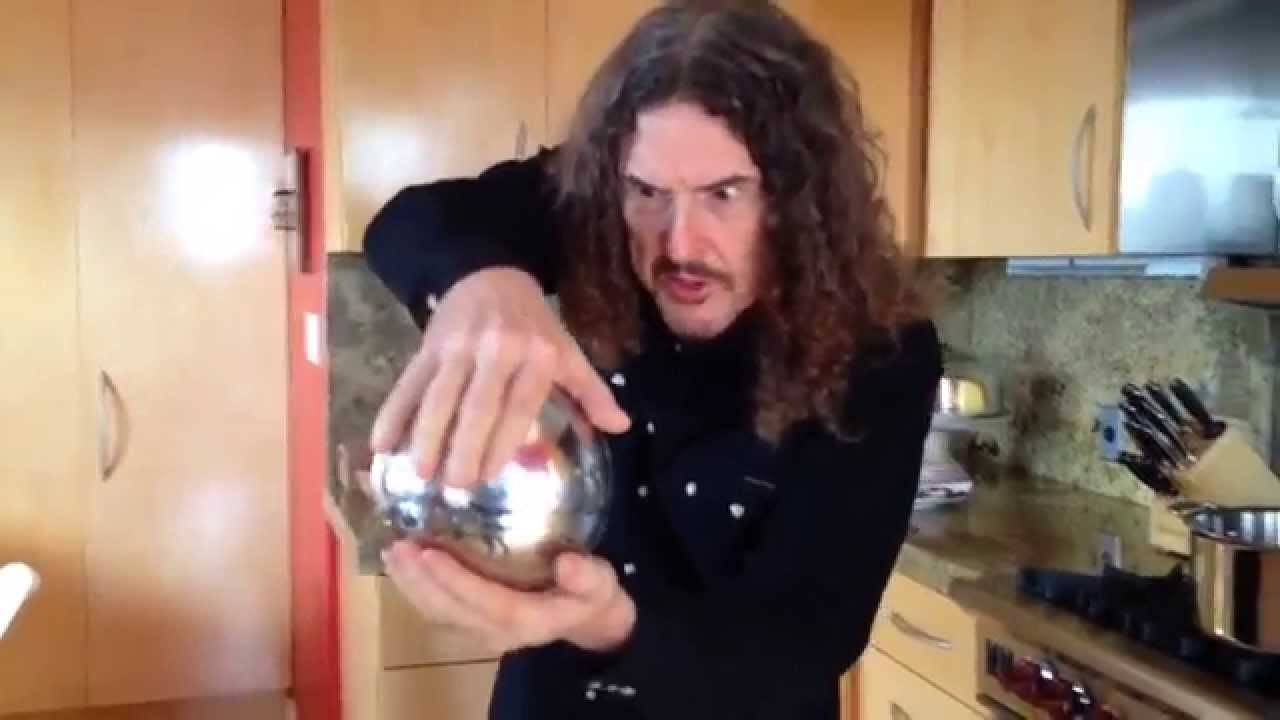
\includegraphics[height=5cm,width=1\textwidth,keepaspectratio]{resources/projection_video.jpg}}
        \label{fig:resources/projection_video.jpg}
    \end{figure}
\end{frame}

\begin{frame}[t]{Projections}
    \framesubtitle{}
    \vspace{-0.3cm}
    On the one hand, we cannot accurately show curved surfaces.

    On the other hand, we can draw something absolutely impossible or something possible but unclear.

    \vspace{-0.5cm}

    \begin{figure}[H]
        \centering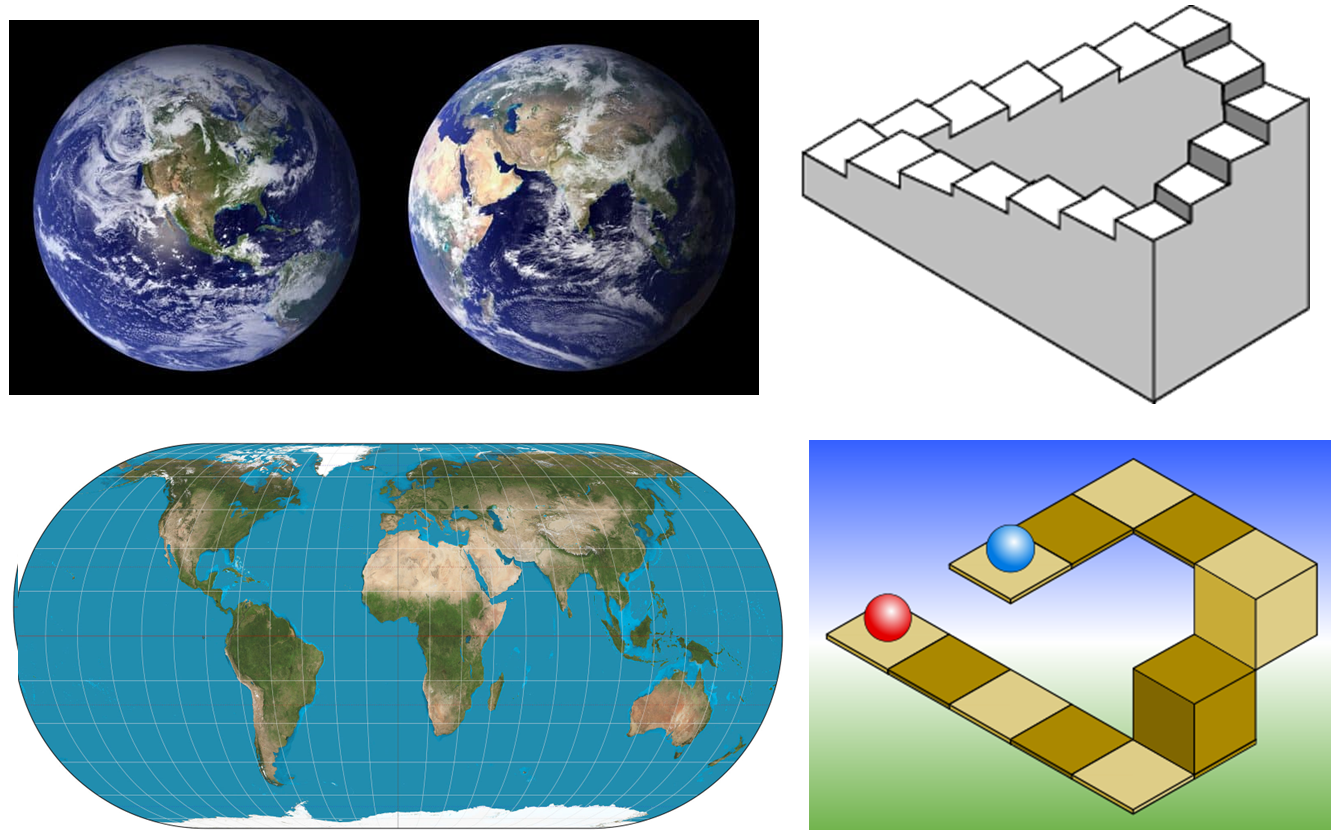
\includegraphics[height=5cm,width=1\textwidth,keepaspectratio]{resources/proj_1.png}
        \label{fig:resources/proj_1.png}
    \end{figure}
\end{frame}

\begin{frame}[t]{Parallel and perspective projections}
    \framesubtitle{}
    \vspace{-0.6cm}
    \begin{figure}[H]
        \centering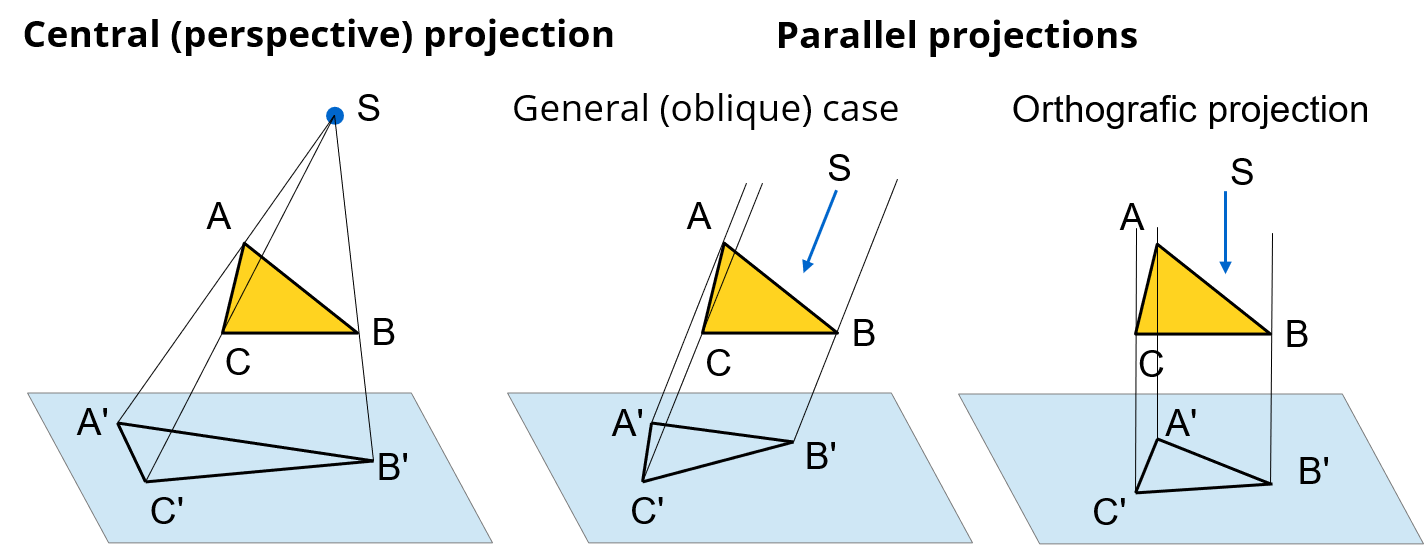
\includegraphics[height=6cm,width=1\textwidth,keepaspectratio]{resources/proj_2.png}
        \label{fig:resources/proj_2.png}
    \end{figure}
\end{frame}

\begin{frame}[t]{Axonometric projections}
    \framesubtitle{General}
    \vspace{-0.6cm}
    \begin{figure}[H]
        \centering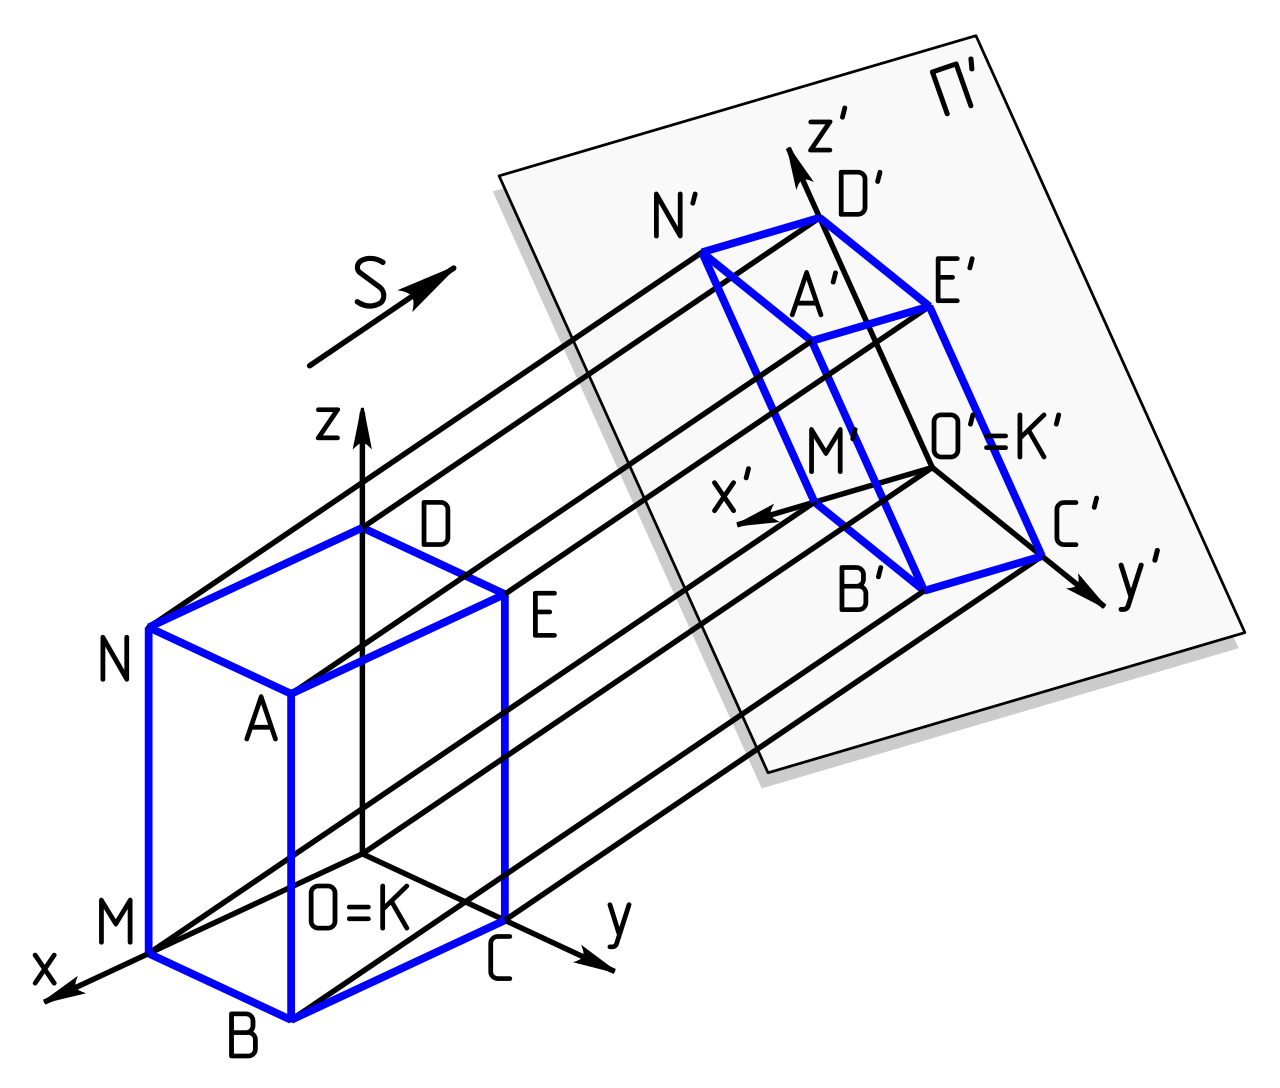
\includegraphics[height=6cm,width=1\textwidth,keepaspectratio]{resources/axono.png}
        \label{fig:resources/axono.png}
    \end{figure}
\end{frame}

\begin{frame}[t]{Axonometric projections}
    \framesubtitle{}
    \vspace{-0.6cm}
    \begin{figure}[H]
        \centering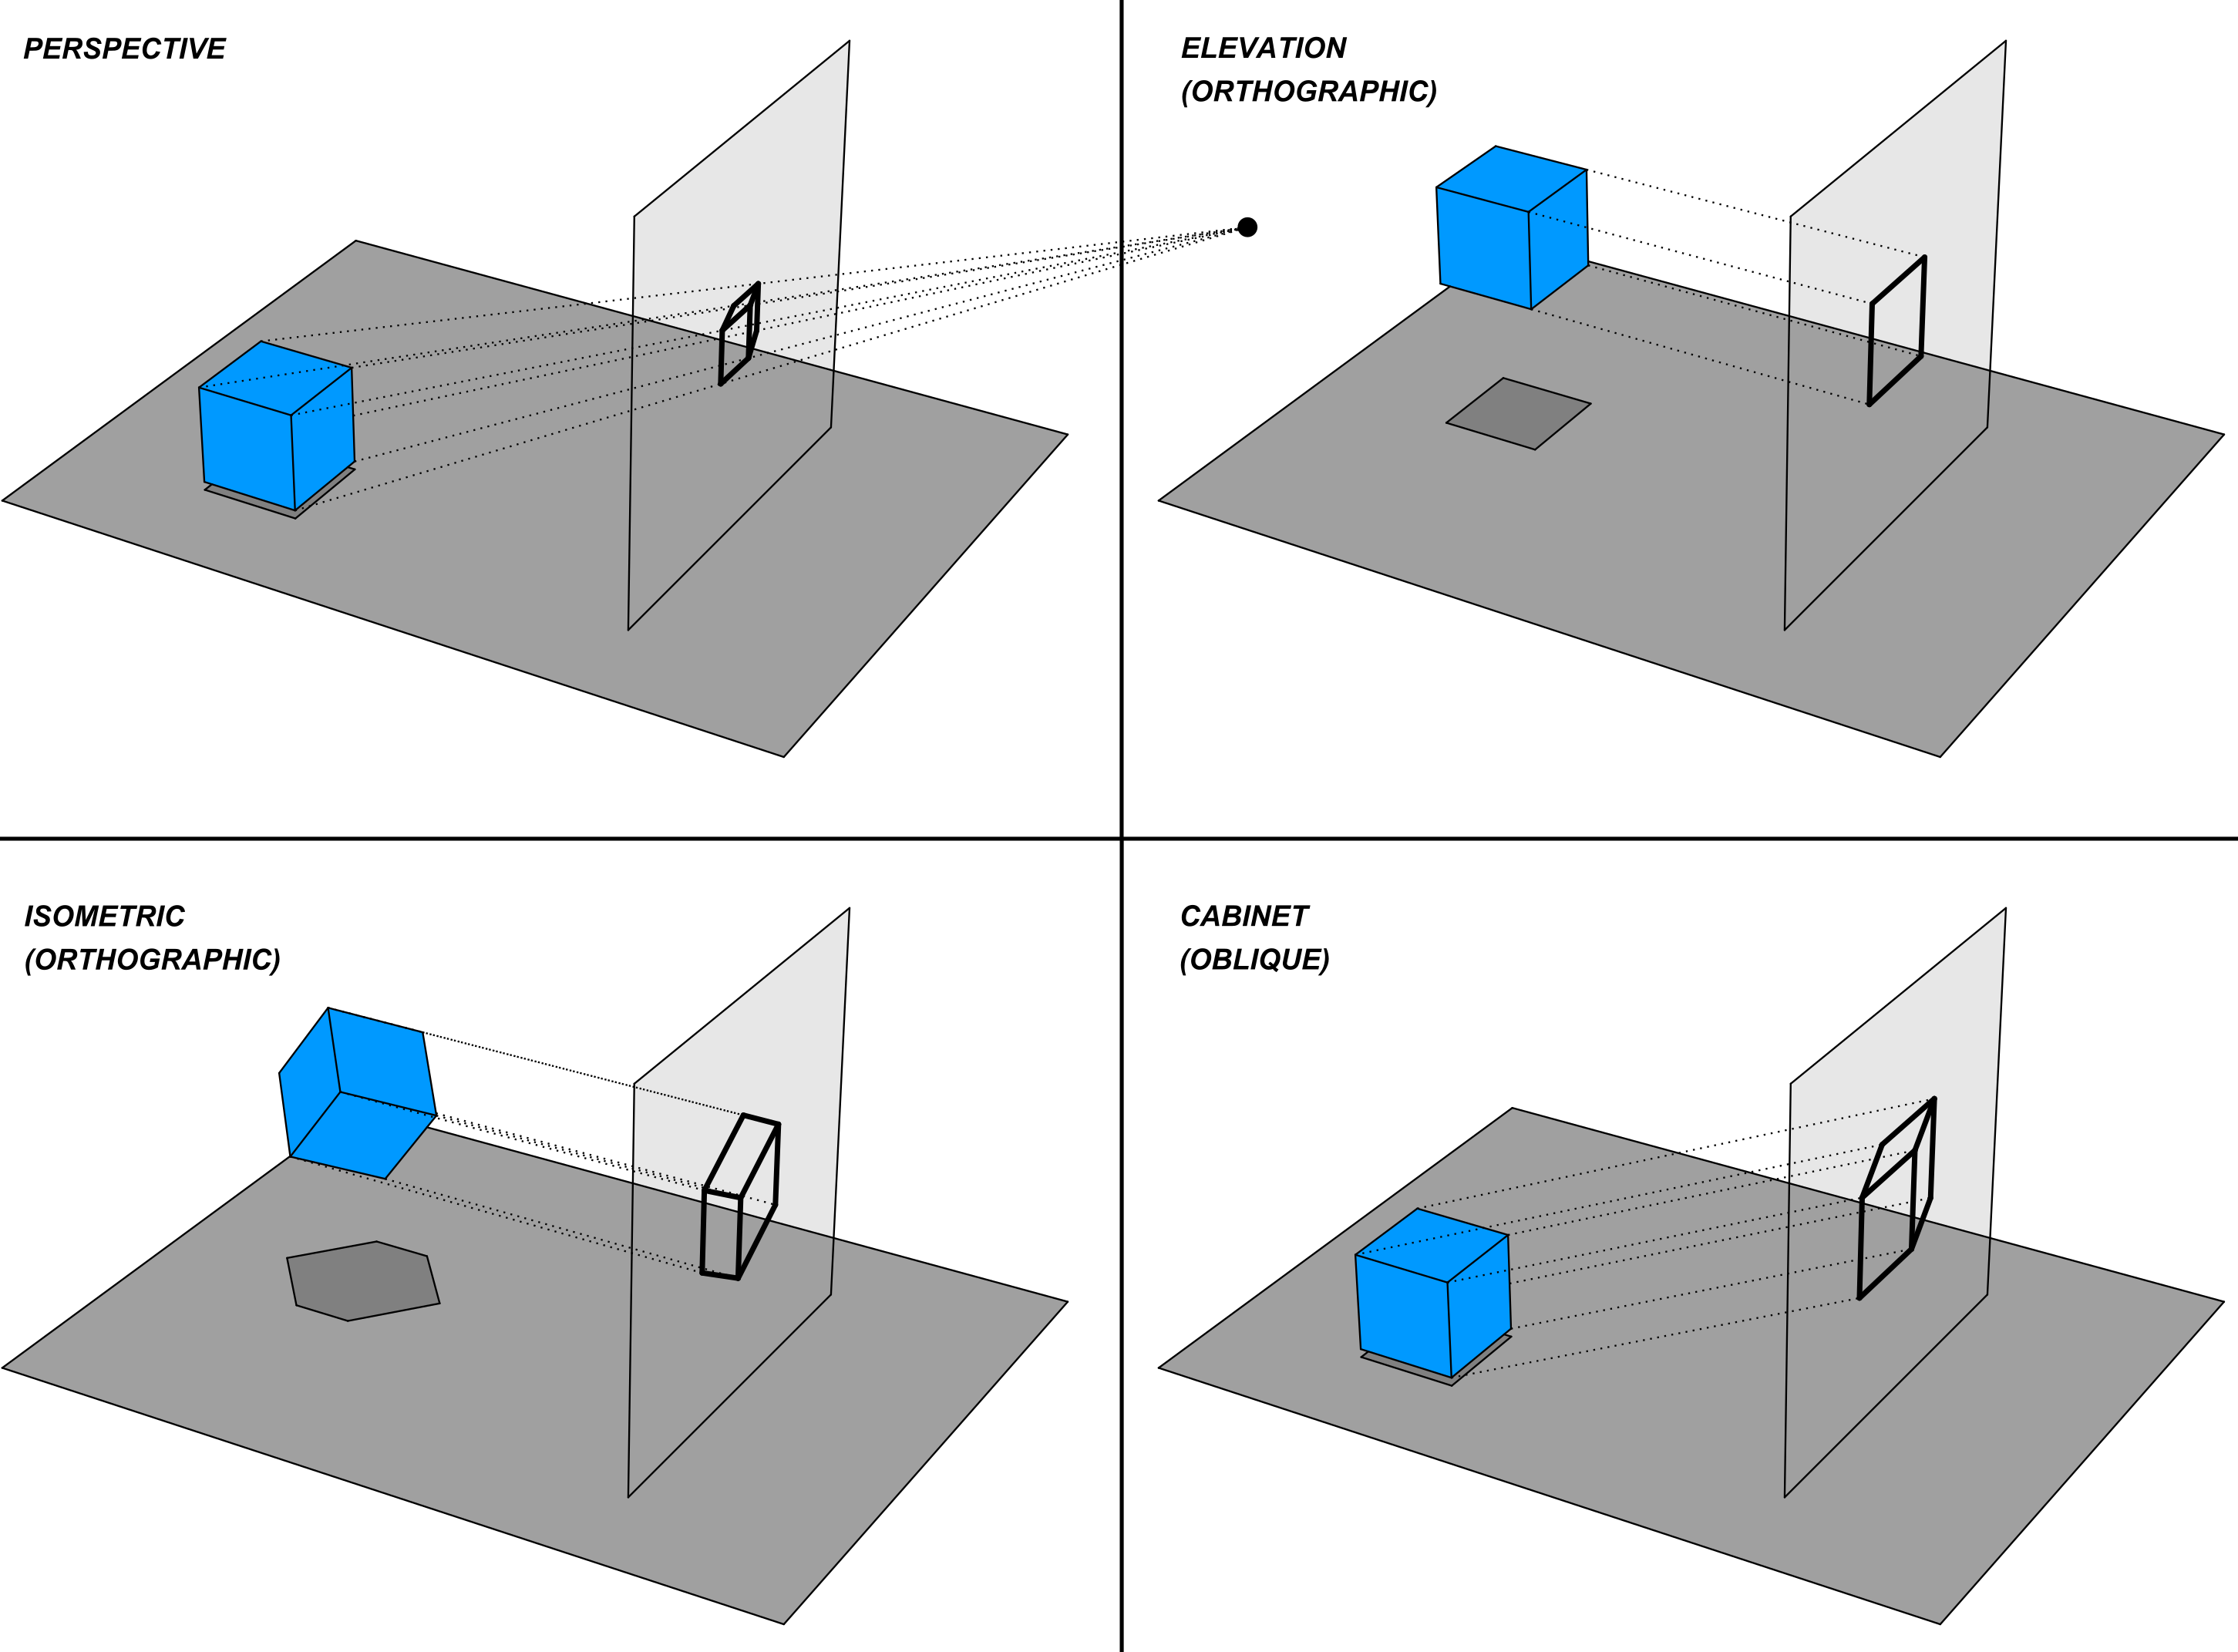
\includegraphics[height=6.5cm,width=1\textwidth,keepaspectratio]{resources/various_proj.png}
        \label{fig:resources/various_proj.png}
    \end{figure}
\end{frame}

\begin{frame}[t]{Axonometric projections}
    \framesubtitle{}
    \vspace{-0.6cm}
    \begin{figure}[H]
        \begin{subfigure}{0.99\textwidth}
            \centering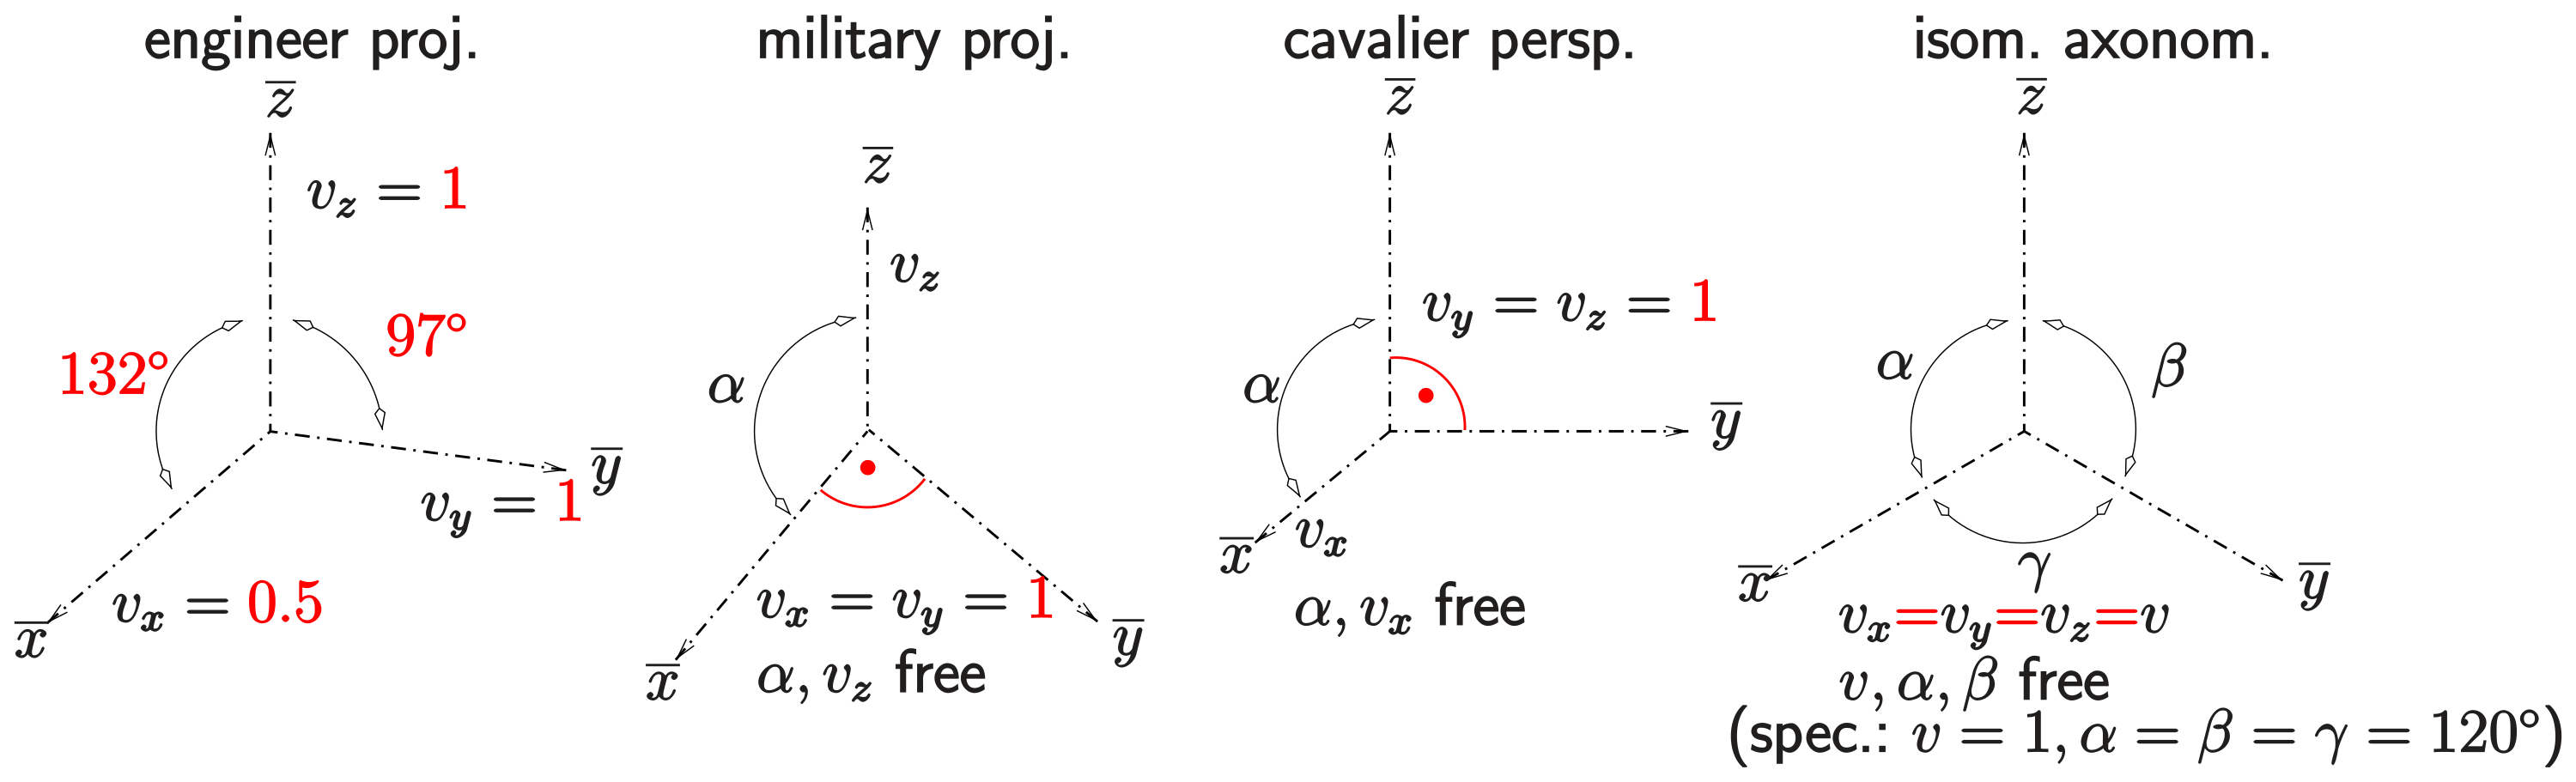
\includegraphics[height=3cm,width=1\textwidth,keepaspectratio]{resources/proj_types_1.png}
            % \caption{capture1}
            \label{fig:resources/proj_types_1.png}
        \end{subfigure}

        \begin{subfigure}{0.99\textwidth}
            \centering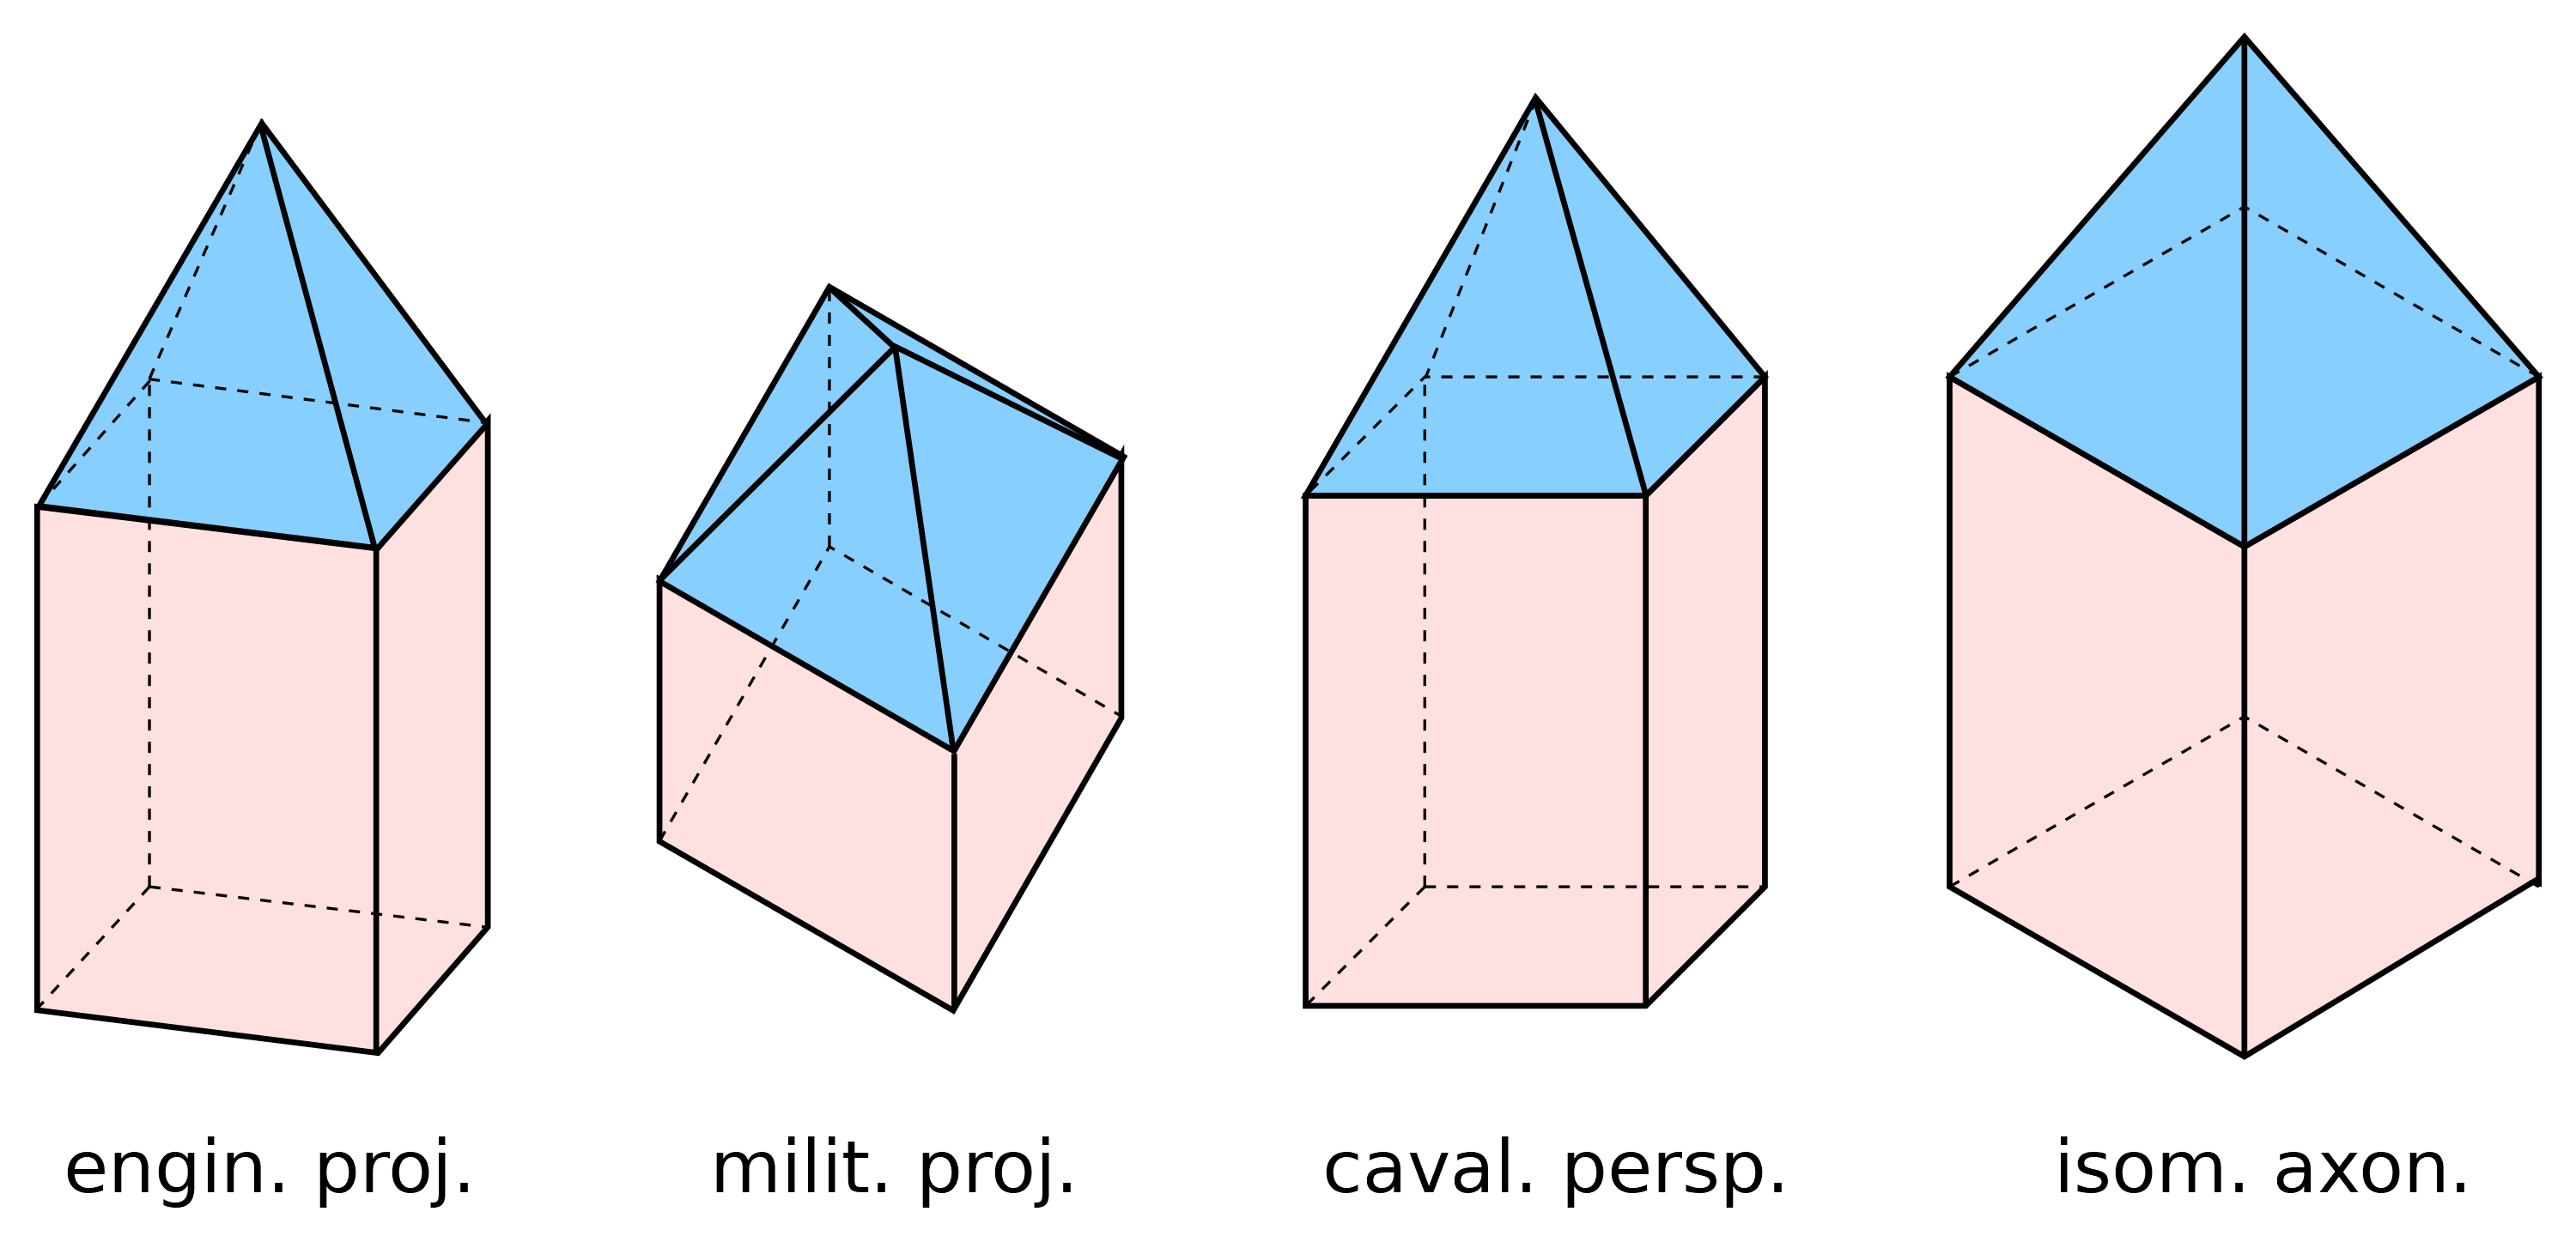
\includegraphics[height=3.5cm,width=1\textwidth,keepaspectratio]{resources/proj_types_2.png}
            % \caption{capture2}
            \label{fig:resources/proj_types_2.png}
        \end{subfigure}
    \end{figure}
\end{frame}

\begin{frame}[t]{Make a line projection}
    \framesubtitle{Video}
    \vspace{-0.6cm}
    \begin{figure}[H]
        \href{https://youtu.be/M21dLeCLWZ8?t=450}{
            \centering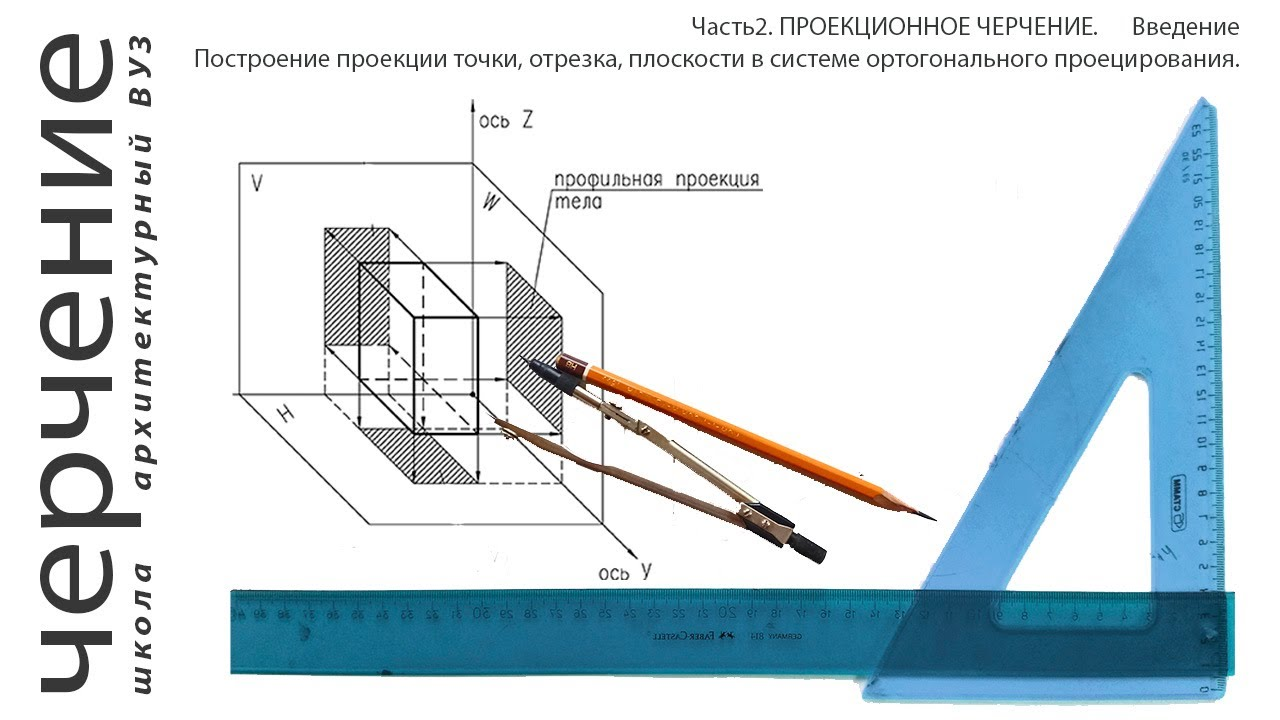
\includegraphics[height=6cm,width=1\textwidth,keepaspectratio]{resources/create_proj_video.jpg}}
        \label{fig:resources/create_proj_video.jpg}
    \end{figure}
\end{frame}

\begin{frame}[t]{Orthographic Multiview projections}
    \framesubtitle{}
    \vspace{-0.6cm}
    \begin{figure}[H]
        \centering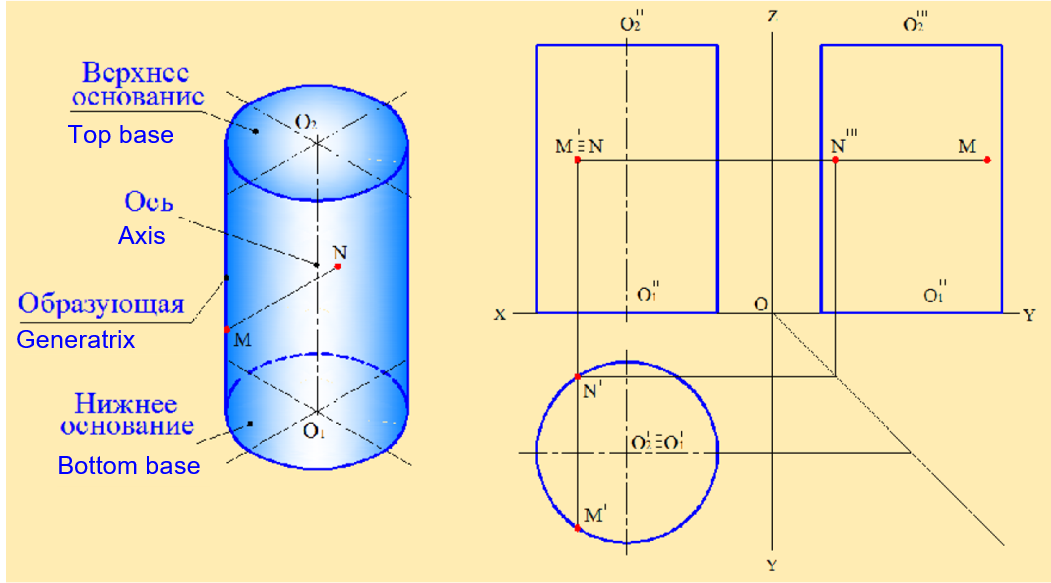
\includegraphics[height=6.5cm,width=1\textwidth,keepaspectratio]{resources/multiview_1.png}
        \label{fig:resources/multiview_1.png}
    \end{figure}
\end{frame}

\begin{frame}[t]{Orthographic Multiview projections}
    \framesubtitle{}
    \vspace{-0.6cm}
    \begin{figure}[H]
        \centering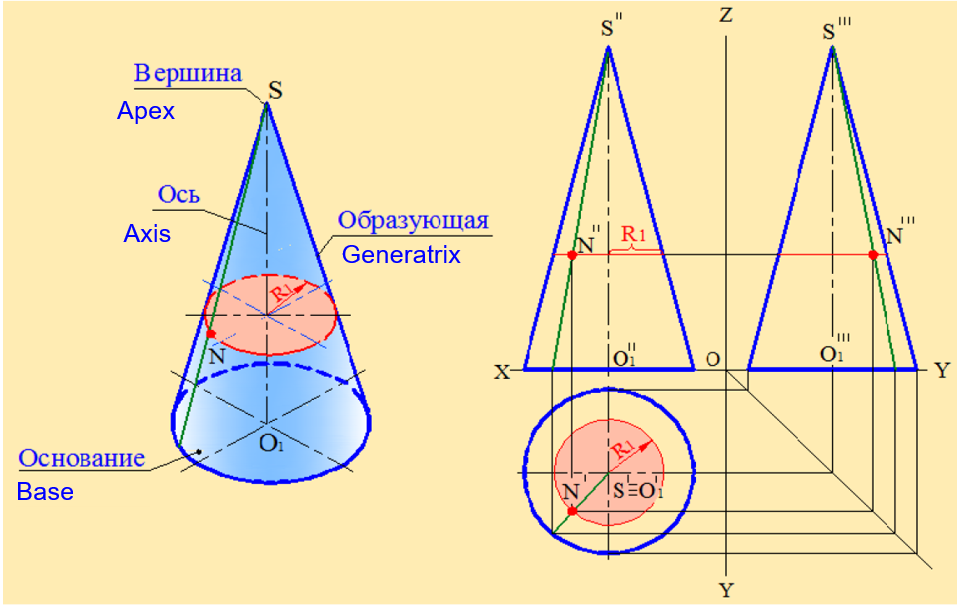
\includegraphics[height=6.5cm,width=1\textwidth,keepaspectratio]{resources/multiview_2.png}
        \label{fig:resources/multiview_2.png}
    \end{figure}
\end{frame}

\begin{frame}[t]{Orthographic Multiview projections}
    \framesubtitle{}
    \vspace{-0.6cm}
    \begin{figure}[H]
        \centering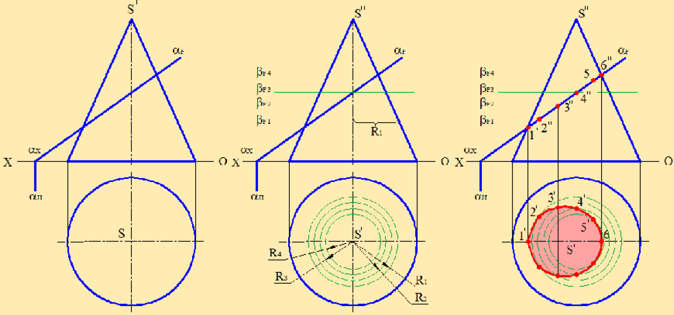
\includegraphics[height=6.5cm,width=1\textwidth,keepaspectratio]{resources/multiview_3.png}
        \label{fig:resources/multiview_3.png}
    \end{figure}
\end{frame}

\begin{frame}[t]{Orthographic Multiview projections}
    \framesubtitle{}
    \vspace{-0.6cm}
    \begin{figure}[H]
        \centering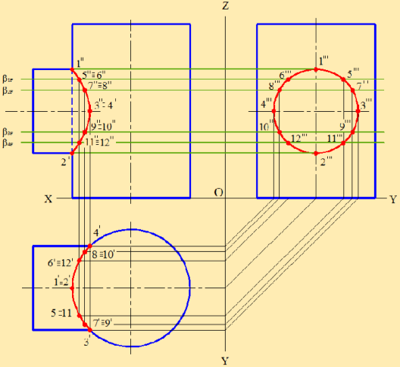
\includegraphics[height=6.5cm,width=1\textwidth,keepaspectratio]{resources/multiview_4.png}
        \label{fig:resources/multiview_4.png}
    \end{figure}
\end{frame}

\begin{frame}[t]{Orthographic Multiview projections}
    \framesubtitle{The difference between European and American standards}
    \vspace{-0.6cm}
    \begin{figure}[H]
        \centering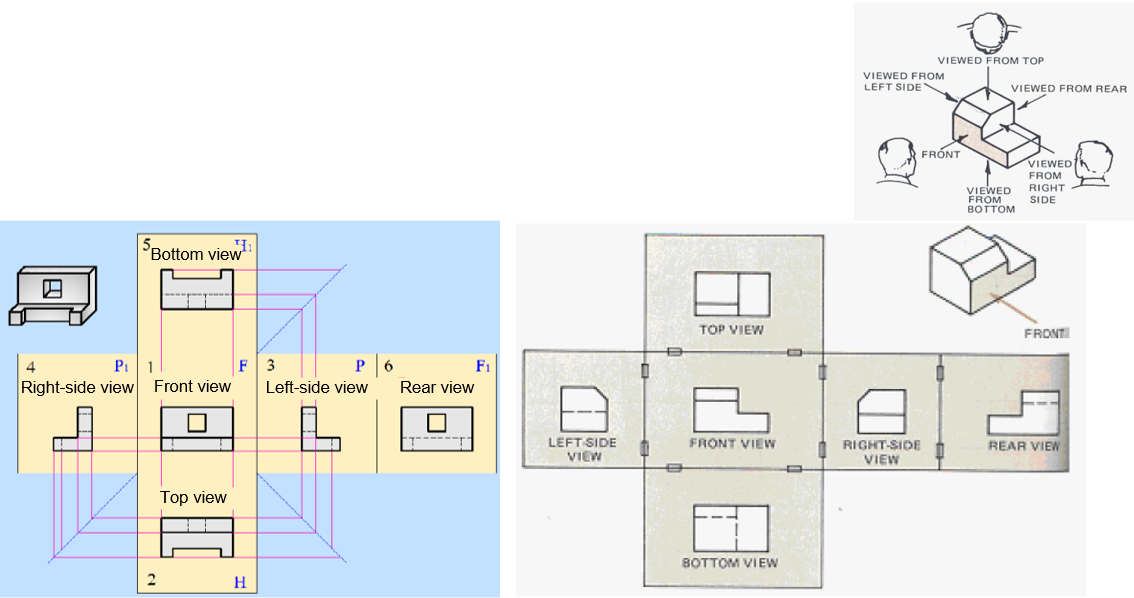
\includegraphics[height=6cm,width=1\textwidth,keepaspectratio]{resources/views.png}
        \label{fig:resources/views.png}
    \end{figure}
\end{frame}

\begin{frame}[t]{Orthographic Multiview projections}
    \framesubtitle{}
    \vspace{-0.6cm}
    \begin{figure}[H]
        \begin{subfigure}{0.49\textwidth}
            \centering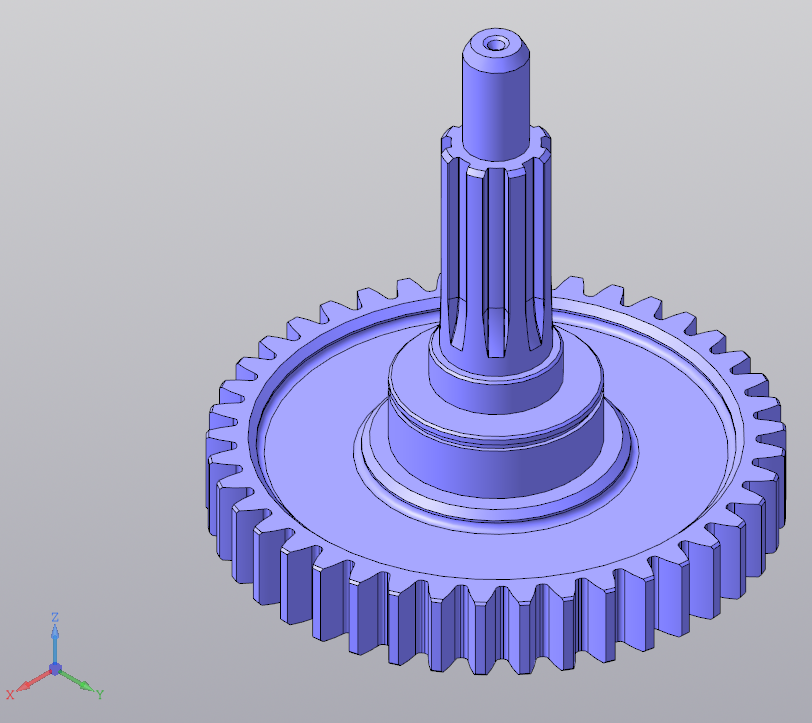
\includegraphics[height=6cm,width=1\textwidth,keepaspectratio]{resources/kompas_1.png}
            \caption*{Kompas 3D}
            \label{fig:resources/kompas_1.png}
        \end{subfigure}
        \begin{subfigure}{0.49\textwidth}
            \centering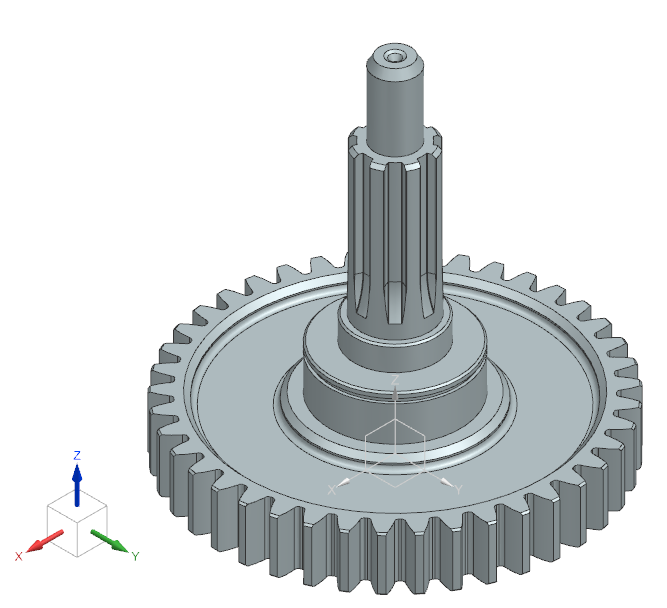
\includegraphics[height=6cm,width=1\textwidth,keepaspectratio]{resources/nx_1.png}
            \caption*{Siemens NX}
            \label{fig:resources/nx_1.png}
        \end{subfigure}
    \end{figure}
\end{frame}

\begin{frame}[t]{Orthographic Multiview projections}
    \framesubtitle{}
    \vspace{-0.6cm}
    \begin{figure}[H]
        \begin{subfigure}{0.49\textwidth}
            \centering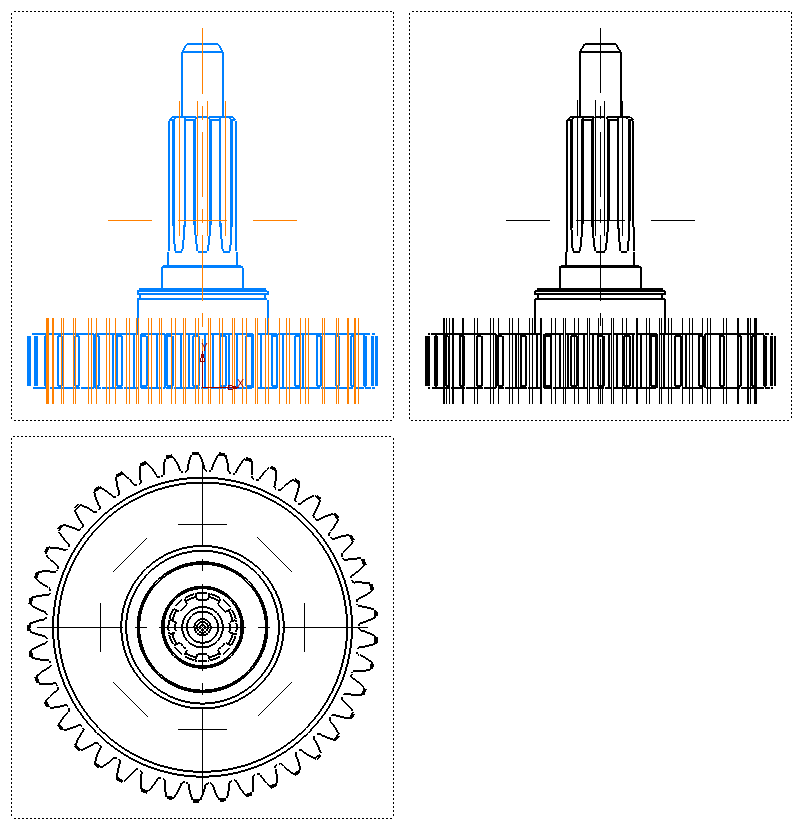
\includegraphics[height=6cm,width=1\textwidth,keepaspectratio]{resources/kompas_2.png}
            \caption*{Kompas 3D (European system)}
            \label{fig:resources/kompas_2.png}
        \end{subfigure}
        \begin{subfigure}{0.49\textwidth}
            \centering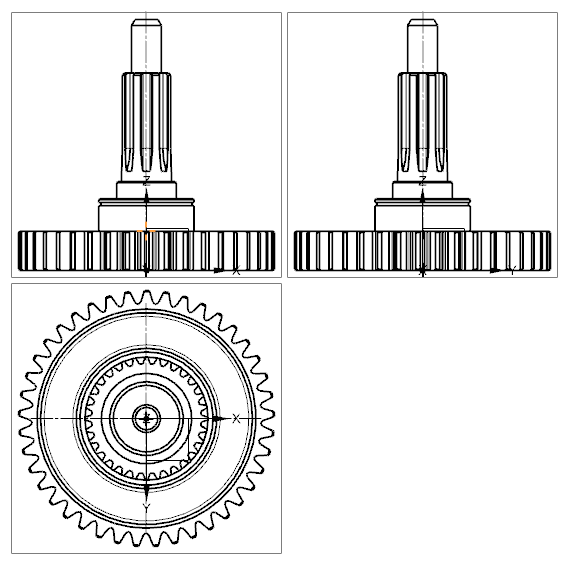
\includegraphics[height=6cm,width=1\textwidth,keepaspectratio]{resources/nx_2.png}
            \caption*{Siemens NX (American system)}
            \label{fig:resources/nx_2.png}
        \end{subfigure}
    \end{figure}
\end{frame}

\begin{frame}[c]{Drawing standards}
    \framesubtitle{}
    \vspace{-0.6cm}
    \begin{figure}[H]
        \begin{subfigure}{0.49\textwidth}
            \centering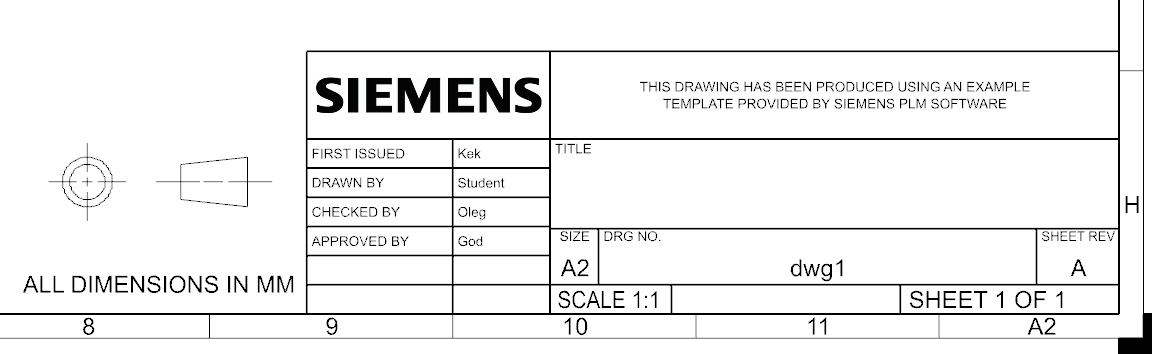
\includegraphics[height=6cm,width=1\textwidth,keepaspectratio]{resources/ansi.png}
            \caption*{ANSI standard Title Block}
            \label{fig:resources/ansi.png}
        \end{subfigure}
        \begin{subfigure}{0.49\textwidth}
            \centering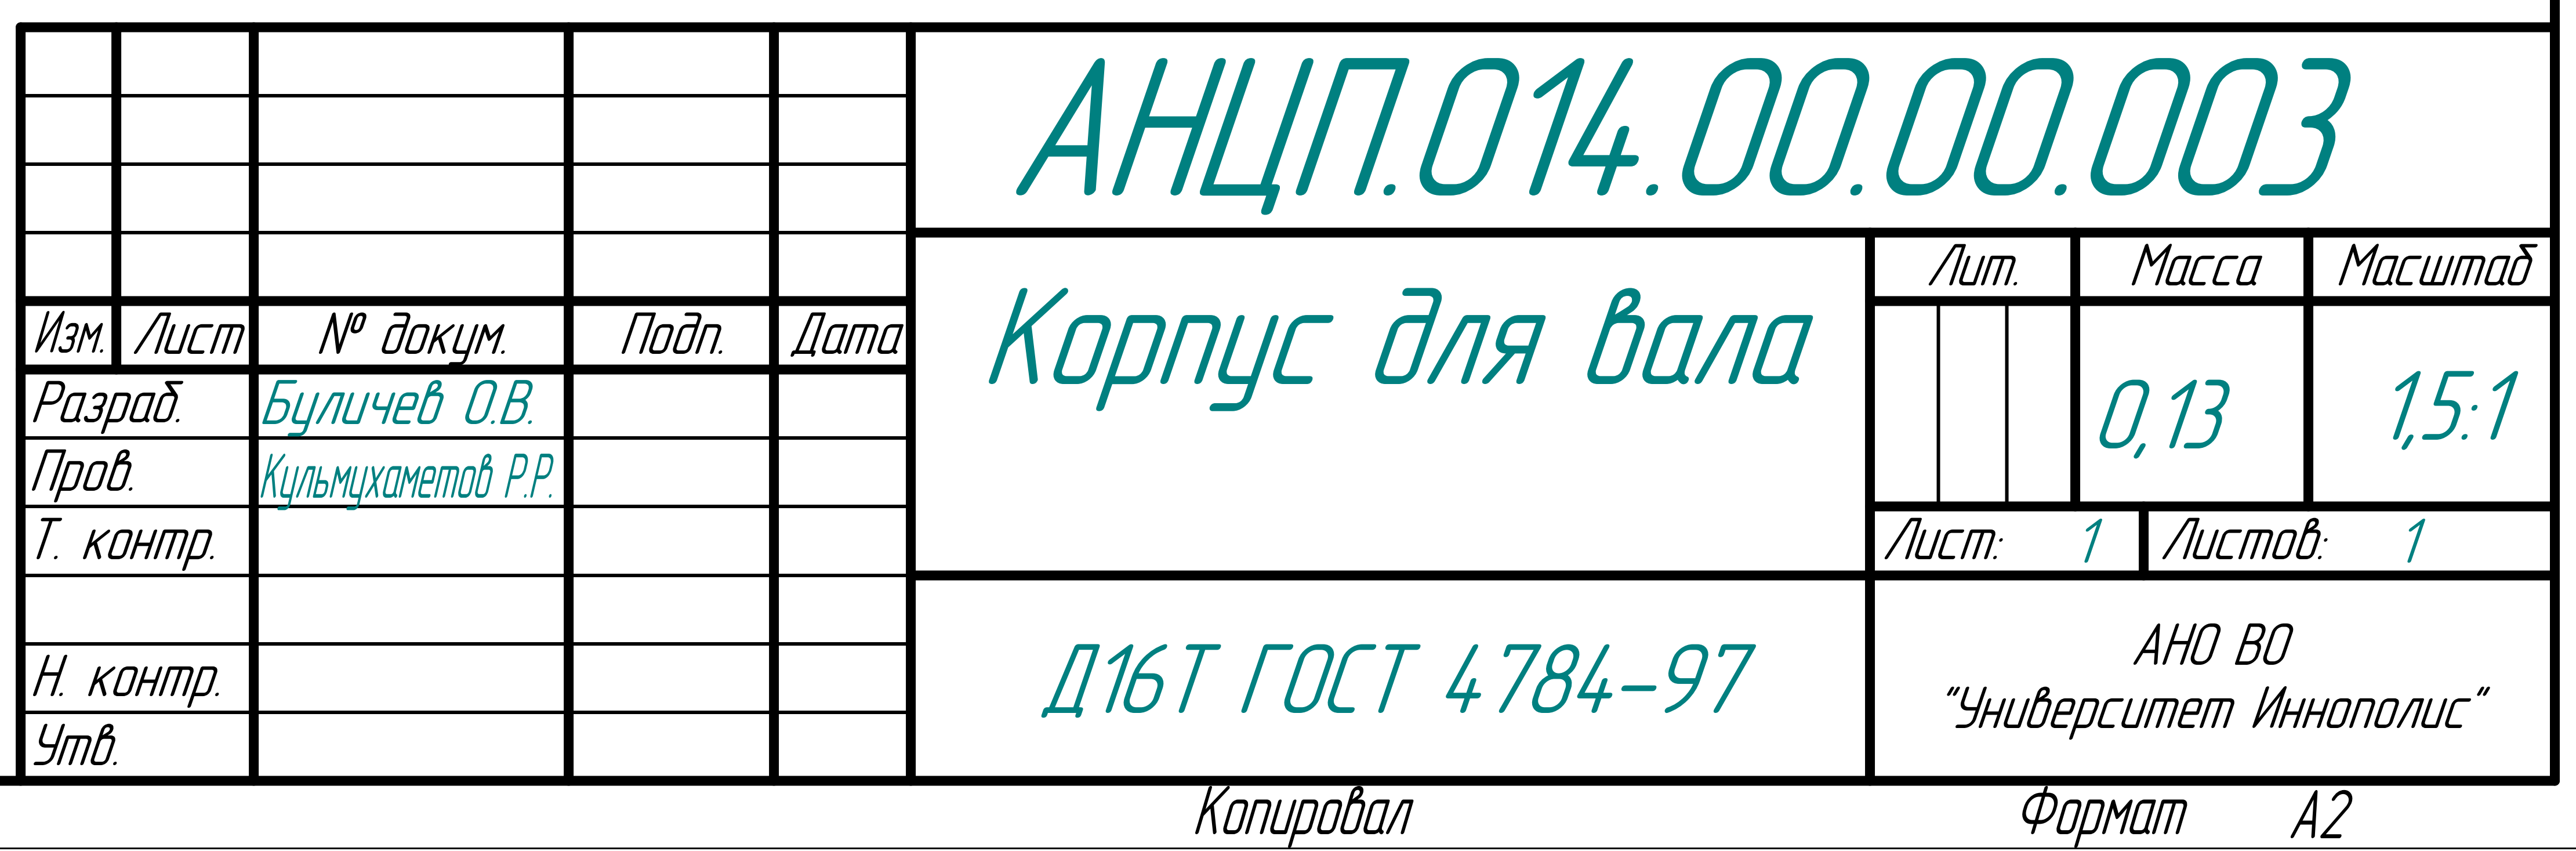
\includegraphics[height=6cm,width=1\textwidth,keepaspectratio]{resources/gost.png}
            \caption*{\textbf{GOST} standard Title Block}
            \label{fig:resources/gost.png}
        \end{subfigure}
    \end{figure}
\end{frame}

\begin{frame}[t]{GOST Drawing Example}
    \framesubtitle{}
    \vspace{-0.6cm}
    \begin{figure}[H]
        \centering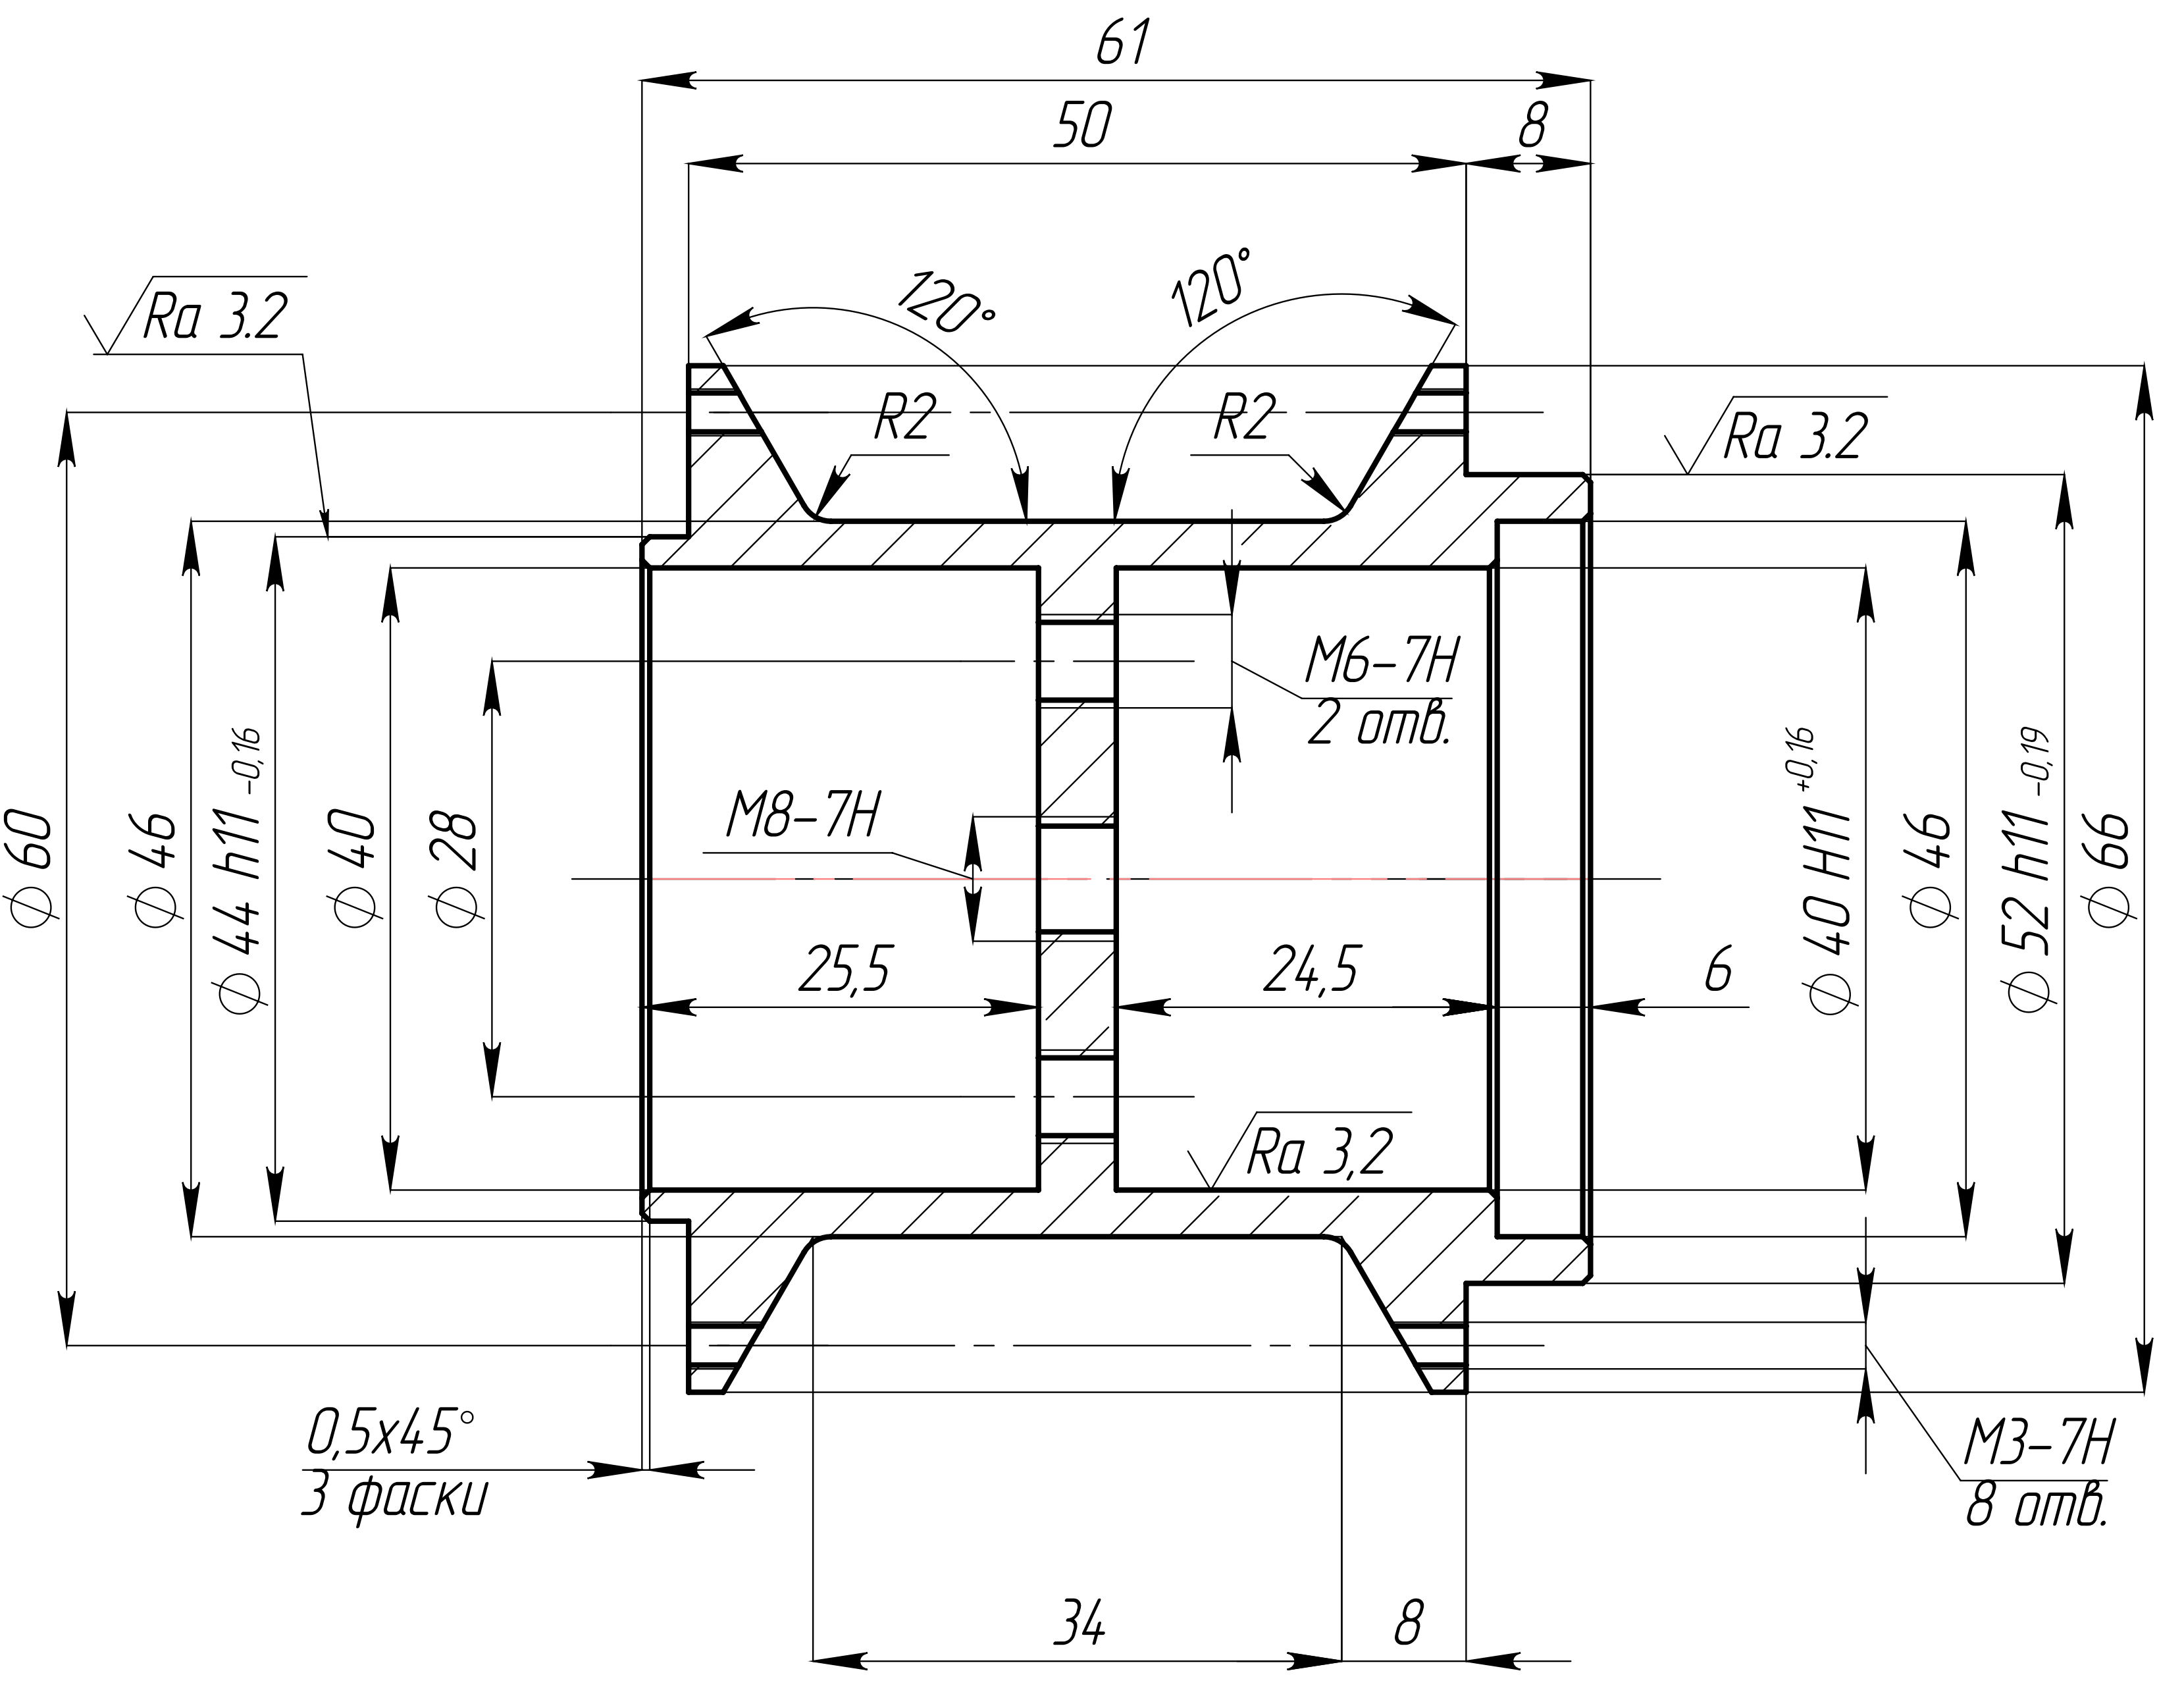
\includegraphics[height=6.5cm,width=1\textwidth,keepaspectratio]{resources/example_gost.png}
        \label{fig:resources/example_gost.png}
    \end{figure}
\end{frame}

\begin{frame}[t]{GOST Drawings}
    \framesubtitle{}
    \vspace{-0.6cm}
    \begin{figure}[H]
        \centering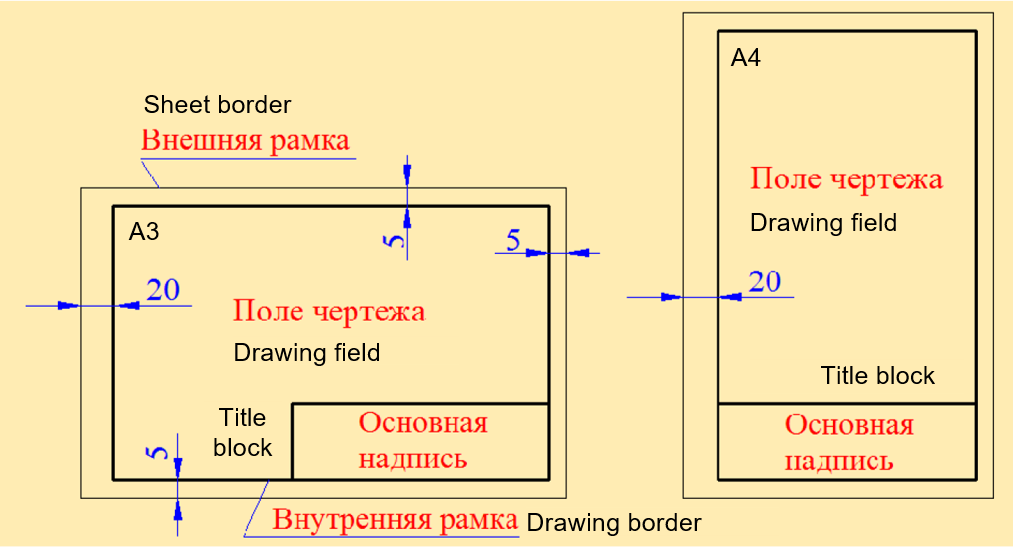
\includegraphics[height=6cm,width=1\textwidth,keepaspectratio]{resources/title_block.png}
        \label{fig:resources/title_block.png}
    \end{figure}
\end{frame}

\begin{frame}[t]{GOST Drawing Title Block}
    \framesubtitle{}
    \vspace{-0.6cm}
    \begin{figure}[H]
        \centering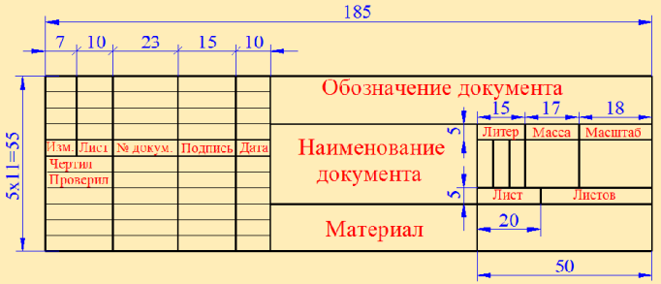
\includegraphics[height=6cm,width=1\textwidth,keepaspectratio]{resources/title.png}
        \label{fig:resources/title.png}
    \end{figure}
\end{frame}

\begin{frame}[t]{Scale}
    \framesubtitle{}
    \vspace{-0.6cm}
    \begin{figure}[H]
        \centering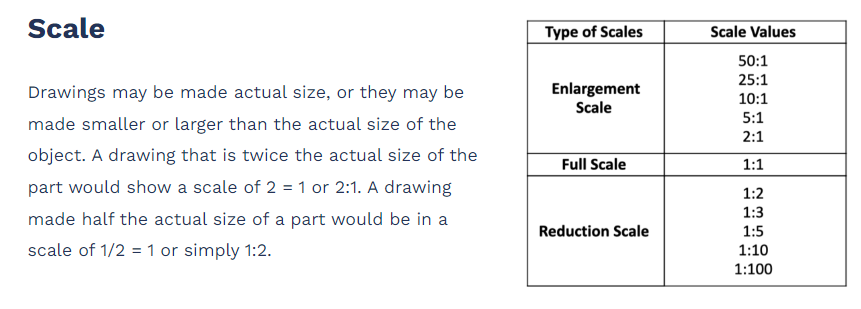
\includegraphics[height=6cm,width=1\textwidth,keepaspectratio]{resources/scale.png}
        \label{fig:resources/scale.png}
    \end{figure}
\end{frame}

\begin{frame}[t]{Type of lines}
    \framesubtitle{}
    \vspace{-0.6cm}
    \begin{figure}[H]
        \centering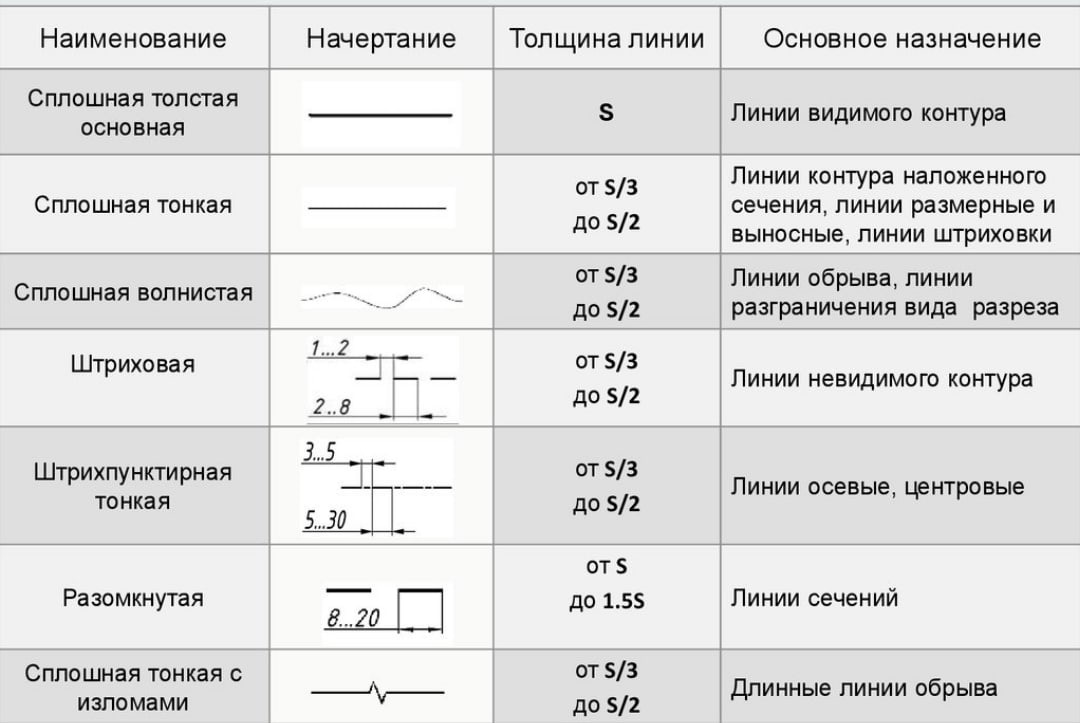
\includegraphics[height=6cm,width=1\textwidth,keepaspectratio]{resources/types_of_lines.jpg}
        \label{fig:resources/types_of_lines.jpg}
    \end{figure}
\end{frame}

\begin{frame}[t]{GOST Standard}
    \framesubtitle{}
    \vspace{-0.6cm}
    \begin{figure}[H]
        \centering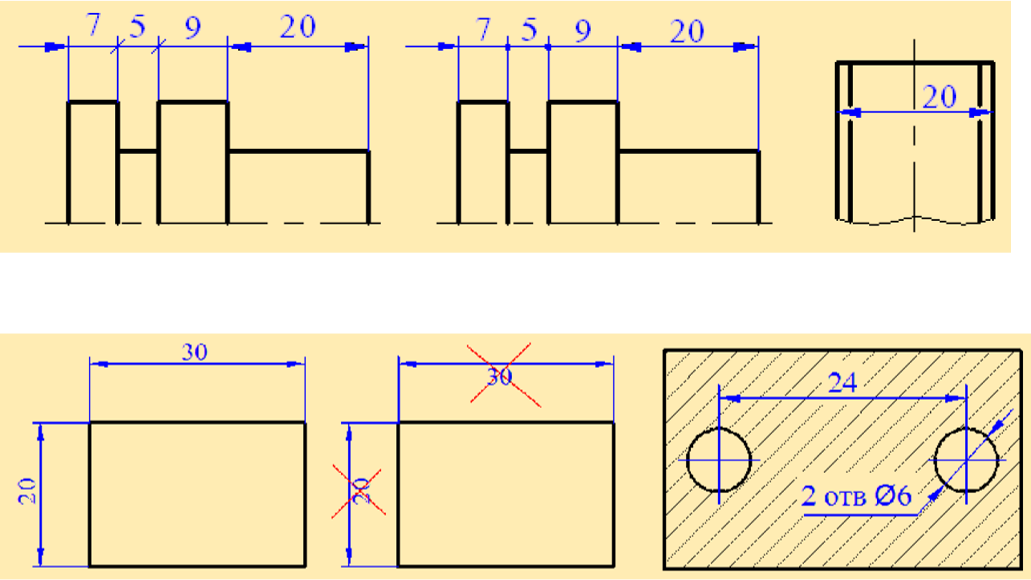
\includegraphics[height=6cm,width=1\textwidth,keepaspectratio]{resources/st1.png}
        \label{fig:resources/st1.png}
    \end{figure}
\end{frame}

\begin{frame}[t]{GOST Standard}
    \framesubtitle{}
    \vspace{-0.6cm}
    \begin{figure}[H]
        \centering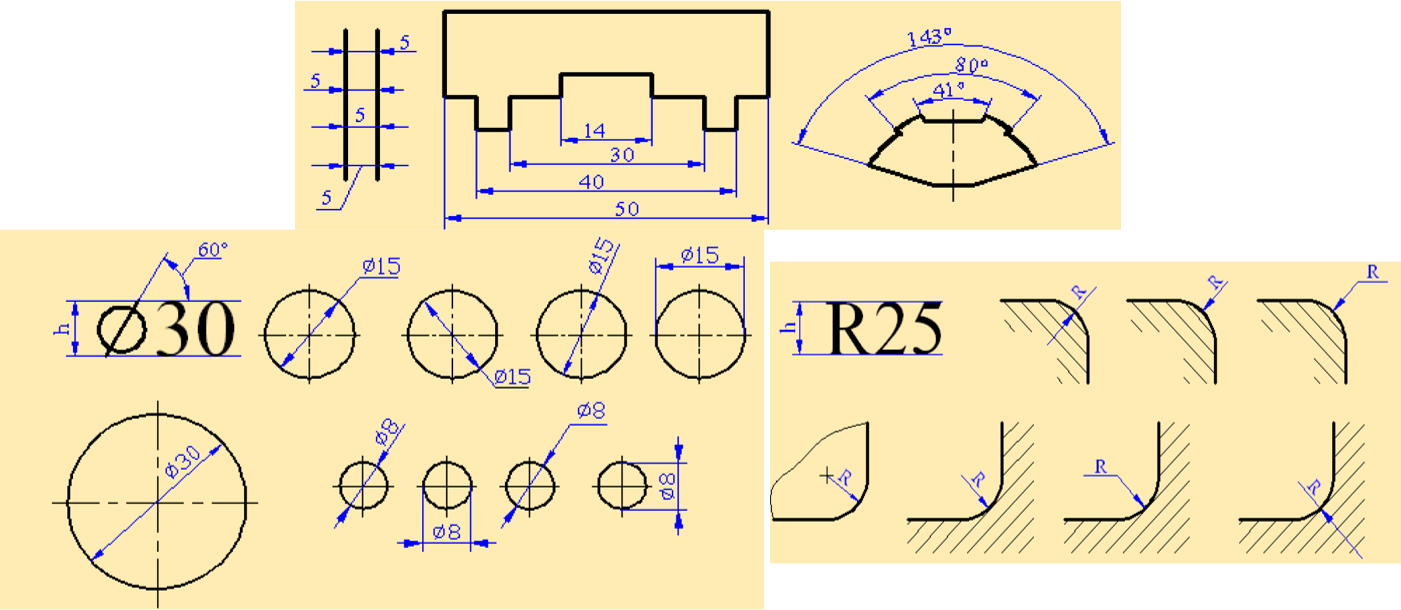
\includegraphics[height=6cm,width=1\textwidth,keepaspectratio]{resources/st2.png}
        \label{fig:resources/st2.png}
    \end{figure}
\end{frame}

\begin{frame}[t]{GOST Standard}
    \framesubtitle{}
    \vspace{-0.6cm}
    \begin{figure}[H]
        \centering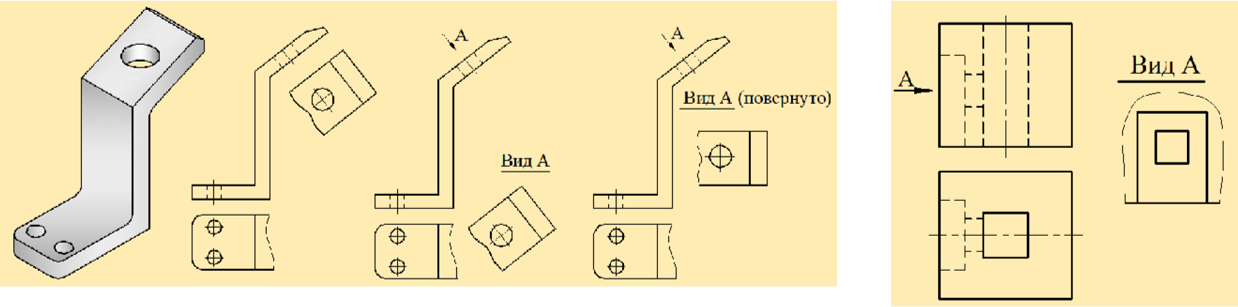
\includegraphics[height=6cm,width=1\textwidth,keepaspectratio]{resources/st3.png}
        \label{fig:resources/st3.png}
    \end{figure}
\end{frame}

\begin{frame}[t]{GOST Standard}
    \framesubtitle{}
    \vspace{-0.6cm}
    \begin{figure}[H]
        \centering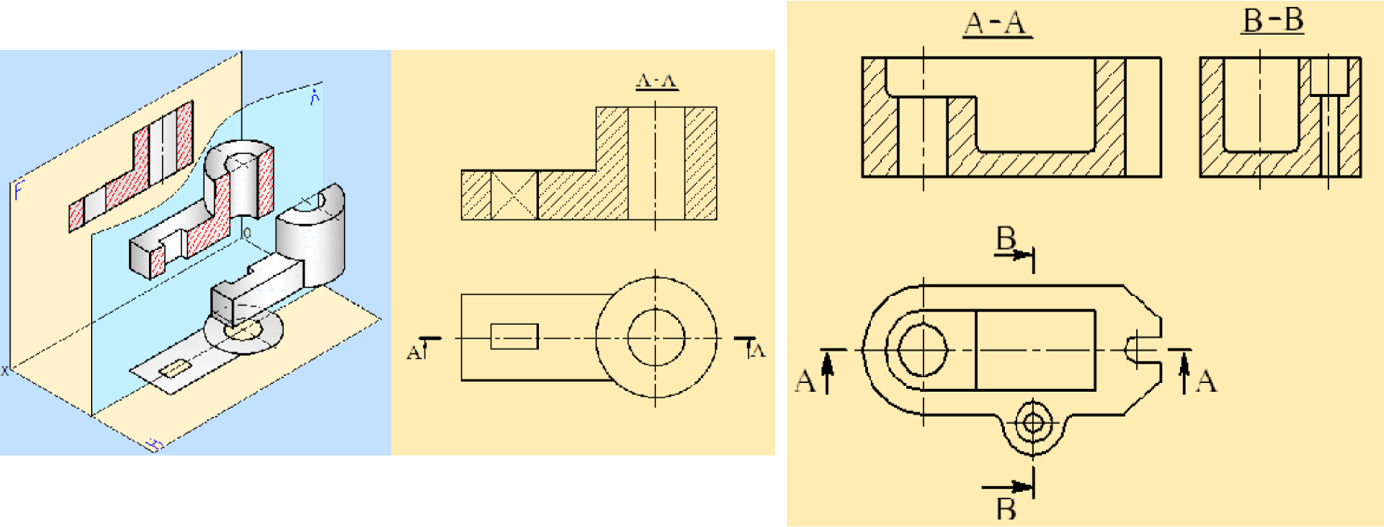
\includegraphics[height=6cm,width=1\textwidth,keepaspectratio]{resources/st4.png}
        \label{fig:resources/st4.png}
    \end{figure}
\end{frame}

\begin{frame}[t]{GOST Standard}
    \framesubtitle{}
    \vspace{-0.6cm}
    \begin{figure}[H]
        \centering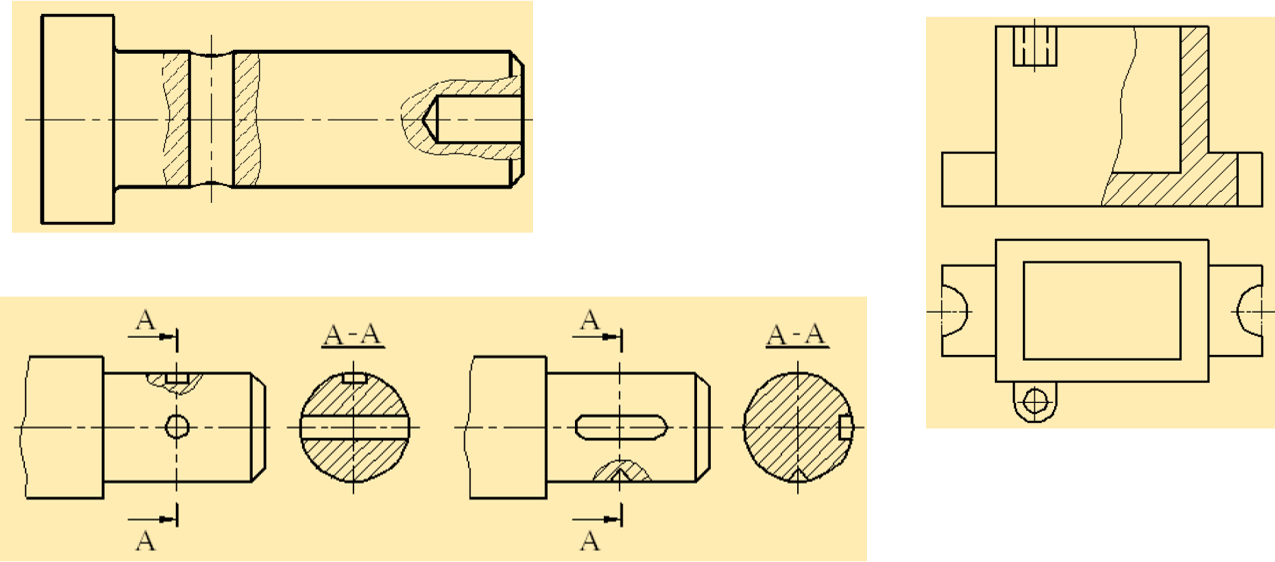
\includegraphics[height=6cm,width=1\textwidth,keepaspectratio]{resources/st5.png}
        \label{fig:resources/st5.png}
    \end{figure}
\end{frame}

\begin{frame}[t]{GOST Standard}
    \framesubtitle{}
    \vspace{-0.6cm}
    \begin{figure}[H]
        \centering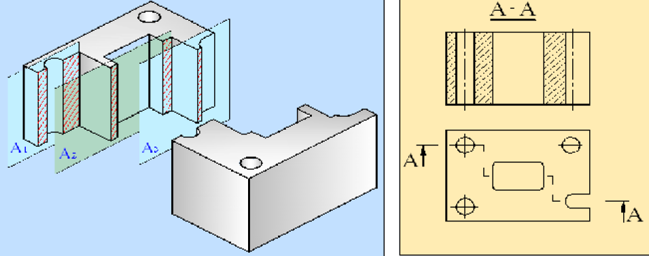
\includegraphics[height=6cm,width=1\textwidth,keepaspectratio]{resources/st6.png}
        \label{fig:resources/st6.png}
    \end{figure}
\end{frame}

\begin{frame}[t]{GOST Standard}
    \framesubtitle{}
    \vspace{-0.6cm}
    \begin{figure}[H]
        \centering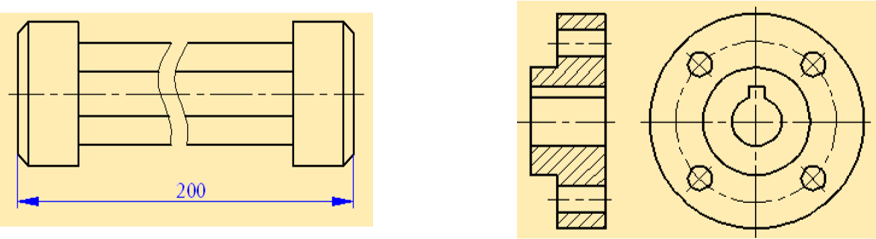
\includegraphics[height=6cm,width=1\textwidth,keepaspectratio]{resources/st7.png}
        \label{fig:resources/st7.png}
    \end{figure}
\end{frame}

\begin{frame}[t]{GOST Standard}
    \framesubtitle{}
    \vspace{-0.6cm}
    \begin{figure}[H]
        \centering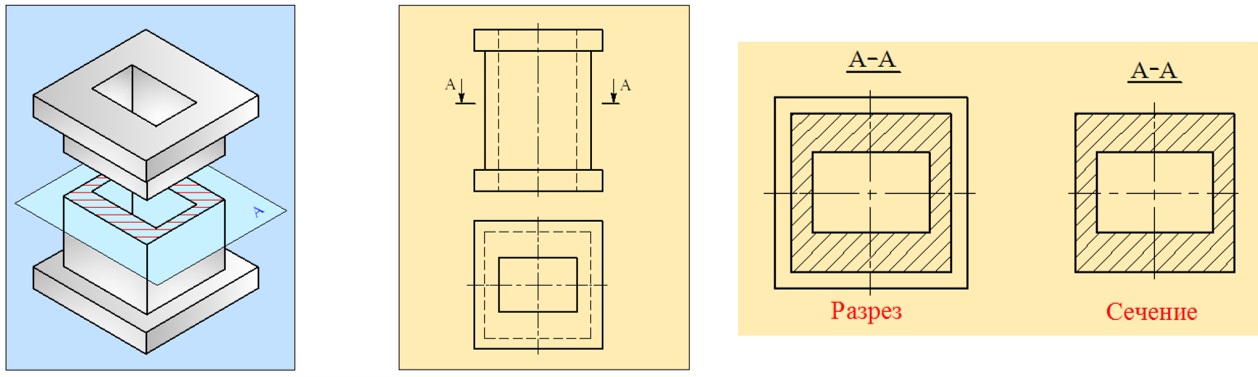
\includegraphics[height=6cm,width=1\textwidth,keepaspectratio]{resources/st8.png}
        \label{fig:resources/st8.png}
    \end{figure}
\end{frame}

\begin{frame}[t]{Understanding Engineering Drawings}
    \framesubtitle{Video}
    \vspace{-0.6cm}
    \begin{figure}[H]
        \href{https://youtu.be/ht9GwXQMgpo}{
            \centering\includegraphics[height=6cm,width=1\textwidth,keepaspectratio]{resources/drawings_video.jpg}}
        \label{fig:resources/drawings_video.jpg}
    \end{figure}
\end{frame}


\begin{frame}[t]{Reference Materials}
    \framesubtitle{}
    \begin{enumerate}
        \item \href{https://werk24.io/knowledge-base-technical-drawings/title-block}{Title Block}
        \item \href{https://thepresentation.ru/grafika/vvedenie-metody-proetsirovaniya-tochka-proetsirovanie-tochki}{Методы проецирования (RUS)}
        \item \href{https://studfile.net/preview/3366860/page:6/}{Инженерная графика (RUS)}
    \end{enumerate}
\end{frame}


\fbckg{fibeamer/figs/last_page.png}
\frame[plain]{}

\end{document}